\documentclass[a4paper,12pt]{article}

\usepackage{amsmath,graphicx,fullpage,microtype,hyperref,subfig,hypcap,amsfonts,parskip}
\usepackage{titlesec}

\titlespacing\section{0pt}{20pt plus 4pt minus 2pt}{2pt plus 4pt minus 2pt}
\titlespacing\subsection{0pt}{16pt plus 4pt minus 2pt}{2pt plus 4pt minus 2pt}

\widowpenalty=400
\clubpenalty=400
\hyphenpenalty=400
\interfootnotelinepenalty=400
\DisableLigatures{encoding=*,family=*}
\numberwithin{equation}{section}
\hypersetup{colorlinks,citecolor=black,filecolor=black,linkcolor=black,urlcolor=black}

\begin{document}

\label{sec:Cover Page}
%\addcontentsline{toc}{section}{Cover Page}

Laurens Bogaardt \hfill \href{http://www.imperial.ac.uk}{Imperial College London}\\
\href{mailto:laurens.bogaardt12@imperial.ac.uk}{laurens.bogaardt12@imperial.ac.uk} \hfill Master's Thesis\\
 \hfill 20-09-2013\\

\vspace{5cm}

\begin{center}
\begin{LARGE}
\begin{bf}
Kaluza-Klein Theory in Quantum Gravity
\end{bf}
\end{LARGE}
\end{center}

\vfill

\begin{center}
\begin{minipage}[t]{0.72\textwidth}
\begin{bf}
Abstract
\end{bf}
\vspace{.2cm}
\newline
In this paper, we discuss a method which aims to combine Kaluza-Klein theory with causal-set theory. We start by reviewing various technologies within each of the theories. In particular, we look at the concept of coarse-graining and at two definitions of the Ricci scalar in a causal-set. Using this knowledge, the proposed method manages to define the four-dimensional Ricci scalar, the action of a gauge field and a scalar field by starting with a five-dimensional causal-set. We conclude that the standard Kaluza-Klein process, which unifies electromagnetism with gravity, can also be applied to a causal-set.
\end{minipage}
\end{center}

\vspace{.6cm}

\begin{center}
\begin{minipage}[t]{0.72\textwidth}
\begin{bf}
Acknowledgements
\end{bf}
\vspace{.2cm}
\newline
The author wishes to thank Dr. Leron Borsten for the supervision of this thesis, for his helpful comments and, in particular, for his insight which lead to the definition of the lower-dimensional Ricci scalar.
\end{minipage}
\end{center}

\vspace{.6cm}

\newpage

\phantomsection
\label{sec:Contents}
%\addcontentsline{toc}{section}{Contents}
\renewcommand{\contentsname}{Contents\\} 

\tableofcontents

\newpage

\section{Introduction}
\label{sec:Introduction}
\subsection{Causal-Set Theory}
\label{sec:Causal-Set Theory}

In 1978, Myrheim suggested spacetime may be a partially ordered set of discrete spacetime-elements in which the order characterised the causal relations between elements~\cite{Myrheim1978}. He hypothesised that the continuous manifold was merely an approximation to this discrete set. Furthermore, he believed that the metric, the spacetime-dimension and other macroscopic quantities would emerge as statistical concepts from the causal structure and the counting measure. This is because it has been shown that the causal structure alone can give us the conformal metric. By counting discrete elements, volume information can be recovered. More specifically, he proposed that there was a correspondence between the number of elements in the set and the spacetime volume and between the discrete partial order and the continuous causal structure:
\begin{subequations}
\label{eq:Correspondence}
\begin{gather}
N\longleftrightarrow V \\
x\prec y\longleftrightarrow x\in J^{-}(y)
\end{gather}
\end{subequations}
This idea was taken up by Bombelli et al. who formalised the concept of a causal-set, a locally finite, partially ordered set of spacetime elements~\cite{Bombelli1987}. Such a set $C$ has an order relation $\prec$ which is transitive, acyclic and locally finite:
\begin{subequations}
\label{eq:Axioms}
\begin{gather}
x\prec y\prec z\Longrightarrow x\prec z \\
x\prec y \text{ and } y\prec x\Longrightarrow x=y \\
|[x, y]| < \infty
\end{gather}
\end{subequations}
Two elements which are causally related, and which do not have any other element in between them, are called linked. A $k$-length chain is a group of $k$ elements which all causally proceed each other. An interval $[x, y]$ between two causally related elements $x$ and $y$ is the diamond-shaped region of their overlapping past- and a future-lightcones.

On a macroscopic scale, this discrete set may look like a spacetime if it faithfully embeds into a manifold. What it means to faithfully embed a causal-set into a manifold will be discussed below, in section~\ref{sec:Sprinkling}. Generally, we will then be able to approximate the causal-set by a continuous spacetime and, hopefully, retrieve all the geometric information for this spacetime from the underlying partial order.

There are various reasons to assume that spacetime is fundamentally discrete. From quantum mechanics, we have learned that, at a fundamental level, matter is made of small indivisible quanta. In order to unify quantum mechanics and general relativity, it seems natural to apply the idea of discrete quanta to spacetime. Additionally, this solves certain problems with infinities in physics~\cite{Sorkin1990}. In quantum field theory, for example, infinities arise is many places. In general relativity too, infinities arise in the curvature of black-holes. Furthermore, black-holes have an entropy, and when the value for this entropy is calculated via the standard quantum field theory, it ends up being infinitely large. Positing a discrete nature of spacetime is one way to avoid these specific problems and is a reasonable assumption in a quantum theory of gravity.

For a more in-depth discussion of discrete spacetime, and of causal-sets in particular, the reviews in~\cite{Dowker2005},~\cite{Henson2009} and~\cite{Sorkin2003} are helpful. These also describe various causal-set technologies, some of which we will see in section~\ref{sec:Causal-Set Technologies}.
\vspace{3mm}


\subsection{Kaluza-Klein Theory}
\label{sec:Kaluza-Klein Theory}

That macroscopic quantities can emerge solely from the causal structure of discrete spacetime points is pivotal to causal-set theory. Within Kaluza-Klein theory, it is matter which emerges from the structure of a higher-dimensional geometry. The original idea by Kaluza was that a five-dimensional empty spacetime can be seen as a four-dimensional spacetime with matter~\cite{Overduin1997}~\cite{Bailin1987}~\cite{Zee2013}. He discovered that the five-dimensional metric can contain the usual four-dimensional metric as well as a gauge field and a scalar field. The gauge field can be identified as the electromagnetic potential $A_\mu$ and its equations of motion in the four-dimensional spacetime reduce to the Maxwell equations. By adding a fifth spacetime dimension, the electromagnetic field can be considered to arise from pure geometry. Electromagnetism is then merely a component of gravity. In this sense, Kaluza unified gravity and electromagnetism, as well as matter and geometry.

In order for the fifth dimension to be undetectable, such that we would only observe our usual four-dimensional spacetime, Kaluza had to impose the 'cylinder condition'. This meant that none of the equations of motion depended on the derivative of the fifth coordinate. Essentially, this boils down to viewing the four-dimensional spacetime as a hypersurface within a five-dimensional world. All of physics would be contained in, and constrained to, that hypersurface. Klein's contribution was to change this view into a more realistic, less artificial picture of nature. He argued that if the fifth dimension was compactified and small, its existence would go unnoticed on all but the highest energy scales. It would be possible that the fifth dimension truly existed, but that present-day experiments were simply not capable of detecting it.

Let us see how this works exactly by considering a field $\psi$ in such a five-dimensional spacetime. We will see that basic quantum mechanics then dictates the cylinder condition must hold, i.e. it leads to an independence from the derivatives of the fifth coordinate. Given that one of the dimensions is now compactified, our field $\psi$ becomes periodic, $\psi(x_0,...,x_3,x_5)=\psi(x_0,...,x_3,x_5+2 \pi r)$, where $r$ is the radius of the compactified circle. Therefore, we can Fourier-expand the field:
\begin{equation}
\label{eq:Fourier}
\psi(x_0,...,x_3,x_5)=\sum_{n=-\infty}^{\infty} \psi_{n}(x_0,...,x_3) e^{\frac{i n x_5}{r}}
\end{equation}
The $\psi_n$'s are the Fourier-modes of the field, each of which carries a momentum in the $x_5$-direction of the order $p_n \sim \frac{|n|}{r}$. If we assume, as Klein did, that the radius $r$ is very small, then these momenta are huge, even for the low $n=1$ mode. In that case, no low-energy experiment would see a field with a derivative of the fifth coordinate. Hence, we would not be able to detect the existence of the fifth dimension at all. We can even choose to ignore the massive modes completely and truncate to the massless sector. Only the $n=0$ mode remains, which is independent of $x_5$. As such, the idea of compactifying the additional dimension automatically leads to Kaluza's cylinder condition. In section~\ref{sec:Kaluza-Klein Technologies} below, we will see that this procedure can, indeed, describe matter fields within a lower-dimensional, continuous spacetime.


\subsection{Matter Fields on Causal-Sets}
\label{sec:Matter Fields on Causal-Sets}

Having replaced the manifold description of spacetime with a causal-set, it is natural to ask how matter fields and their dynamics, normally tied to the continuum formalism, arise within causal-set theory. One attempt by Sverdlov has been to rewrite the Lagrangian for various fields in terms of the causal structure~\cite{Sverdlov2009}. It is the causal structure, and its related concepts such as spacetime volume and time-like length, which persist in causal-set theory. As such, these are easy to discretise and allow you to write down a discrete Lagrangian. Using this procedure, Sverdlov was able to define scalar fields, gauge fields and spinor fields~\cite{Sverdlov2008}~\cite{Sverdlov2008b}~\cite{Sverdlov2008a}. Although the use of the causal structure to define your Lagrangian sounds nice in principle, in practice this results in quite messy expressions. Furthermore, it is a top-down procedure where we might prefer a bottom-up approach.

Another attempt to define matter fields on a causal-set has been by Johnston~\cite{Johnston2010}. This is clearly a bottom-up approach as the field is expressed in terms of the adjacency matrix $A_{C}$ of the set $C$~\cite{Johnston2008}. The adjacency matrix is the most fundamental quantity in causal-set theory and expresses the causal relation between elements. It has entry $1$ on position $ij$ when $v_i \prec v_j$ and $0$ otherwise. One simple property of this matrix is that, when exponentiating it to its $k$th power $A_{C}^{k}$, the entry on position $ij$ provides the number of chains of length $k$ which go from element $v_i$ to element $v_j$. This can be used to define a type of path-integral by assigning an amplitude to every step from one element to the next. Eventually, a geometric matrix series leads to an expression which approximates the continuous retarded Green function~\cite{Johnston2009}. This may then be used to define the discrete Feynman propagator from which a scalar quantum field theory can be built~\cite{Johnston2009a}. This theory can be described in both the operator as well as the sum-over-histories form~\cite{Sorkin2011}. The Johnston propagator can also be defined on non-trivial topologies, such as the surface of a cylinder. It this case, the homotopy matrix is needed to account for the identification of edges of the spacetime~\cite{Schmitzer2010}. In section~\ref{sec:Covering Space} below, we will see how to make use of the homotopy matrix in a another way. Overall, the procedure by Johnston has been successful for a scalar field, and attempts are made to formulate a spinor theory. However, both the approach by Sverdlov and the one by Johnston still rely on matter being added on top of the causal structure.


\subsection{Matter Fields within Causal-Sets}
\label{sec:Matter Fields within Causal-Sets}

Having suggested it is possible for spacetime and geometry to emerge from a set of discrete elements which are causally ordered, it would be nice if all of physics could emerge as a consequence of this order. It would be nice if matter fields themselves followed from the causal-set as a particular structure within the partial order. Then, matter would be an instance of geometry, in the same way as the electromagnetic potential which follows from the five-dimensional geometry in Kaluza-Klein theory. In that case, matter fields would not live on the causal-set, but within it.

So far, there has only been one attempt to define matter fields via a Kaluza-Klein procedure within causal-set theory, done by Sverdlov~\cite{Sverdlov2008b}. In his article, Sverdlov starts off with the discretised four-dimensional Lagrangian for gravity. He then assumes each element of the set is no longer a point, but a circle. He defines the value of the scalar field which arises from the Kaluza-Klein procedure as a function of the portion of a circle-element causally related to another circle-element. He defines the gauge field as a function of the off-center displacement of that causally related portion. Even though it works, this method of obtaining matter fields within a causal-set is rather artificial. It goes against the aim of constructing physics from the simplest entities by assuming all spacetime-points are now circles. It would be preferable if such an artificial assumption was not necessary and if matter fields could emerge solely from a basic causal-set with a particular partial order.

Another approach to combining Kaluza-Klein theory with causal-set theory has been proposed by Jonhston and Surya~\cite{Johnston2010}. They imagined a causal-set which could be approximated by a five-dimensional spacetime with one dimension compactified and small, as in the usual story. One would then write down the Ricci scalar and the Einstein-Hilbert action for this five-dimensional causal-set. As we will see in section~\ref{sec:Kaluza-Klein Technologies} below, it is possible to identify within this five-dimensional action the action for the four-dimensional spacetime, the action for the gauge field and that for the scalar field. It is the purpose of this paper to follow these guidelines and, after reviewing certain technologies which are required for the argument, suggest definitions for the four-dimensional Ricci scalar, the electromagnetic field strength and the dilaton based solely on the causal-set $C$.


\section{Kaluza-Klein Technologies}
\label{sec:Kaluza-Klein Technologies}
\subsection{Metric}
\label{sec:Metric}

We have seen above that there is a simple way to argue for a world with five dimensions, even though we only observe four, via Klein's compactification of the fifth dimension into a small circle of radius $r$. This allows us to write down a five-dimensional metric $\tilde{g}_{MN}$ with $10+4+1=15$ degrees of freedom. We can interpret these variables as corresponding to the original, four-dimensional metric $g_{\mu \nu}$, a gauge field\footnote{As $\tilde{g}_{MN}$ is dimensionless, we should identify $\tilde{g}_{\mu 5}$ with $l A_\mu$ where $l$ sets the normalization of $A_\mu$. However, for simplicity, we absorb this coefficient into the definition of our gauge field. The scalar field is also normalised to obtain the simplest expression.} $A_{\mu}$ and a scalar field $\phi$. There are multiple ways to write down the five-dimensional metric, but a simple way to parametrise it is as follows~\cite{Bailin1987}:
\begin{equation}
\label{eq:Metric}
\tilde{g}_{MN}=\left(\begin{array}{cc}
 g_{\mu \nu}+\phi^2 A_\mu A_\nu & \phi^2 A_\mu \\
\phi^2 A_\nu & \phi^2\\
\end{array}\right)
\end{equation}
We can see that the element $\tilde{g}_{55}$ is basically equal to the value of the scalar field $\phi$, also known as the dilaton~\cite{Zee2013}. The meaning of this is discussed in section~\ref{sec:Dilaton} below, as it will be important in the argument leading up to our causal-set Kaluza-Klein procedure.


\subsection{Ricci Scalar}
\label{sec:Ricci Scalar}

As in the usual four-dimensional case, the action for five-dimensional Einstein gravity in an empty spacetime is simply given by~\cite{Bailin1987}:
\begin{equation}
\label{eq:Five-dimensional action}
\tilde{S}=\int d^5x\sqrt{|\tilde{g}|}\tilde{R}
\end{equation}
Here the tildes signify the higher-dimensional versions of the quantities and, in this case, the Lagrangian is integrated over five variables. By varying the action, the Einstein equations in this five-dimensional empty spacetime can be derived:
\begin{equation}
\label{eq:Einstein equations}
\tilde{G}_{MN}=0
\end{equation}
Using the metric as defined in equation~\ref{eq:Metric} above, invoking Kaluza's cylinder condition by dropping all derivatives of the fifth coordinate and integrating over $x_5$, the Ricci scalar can be evaluated\footnote{The action here is written in the Jordan frame. There is some debate whether it would be better to conformally rescale the metric to the Einstein frame~\cite{Overduin1997}. We will not concern ourselves with that debate here, and continue to work in the Jordan frame, as it proves easier to translate the continuous action to the discrete action in this frame.} in terms of the four-dimensional fields and the effective action may be written down~\cite{Zee2013}:
\begin{equation}
\label{eq:Four-dimensional action}
%S=\int d^4x\sqrt{|g|}\phi (R+\frac{1}{4} \phi^2 F_{\mu \nu } F^{\mu \nu}+\frac{\partial^\alpha \phi \partial_\alpha \phi}{\phi^2})
S=\int d^4x\sqrt{|g|}\phi (R+\frac{1}{4} \phi^2 F_{\mu \nu } F^{\mu \nu}+\frac{\square \phi}{\phi})
\end{equation}
Here, $F_{\mu \nu }=\partial_{\mu} A_{\nu}-\partial_\nu A_{\mu }$ and $\sqrt{|g|}\phi$ replaces the five-dimensional volume-element $\sqrt{|\tilde{g}|}$. Varying this action, we see that the five-dimensional Einstein equations reduce to:
\begin{subequations}
\label{eq:Einstein and Maxwell equations}
\begin{gather}
G_{\mu\nu}=8\pi G\phi^2 T_{\mu \nu}-\frac{1}{\phi}(\nabla_\mu \nabla_\nu \phi -g_{\mu \nu} \square \phi)\\
\nabla^\mu F_{\mu \nu}=-\frac{3}{\phi} \partial^\mu \phi F_{\mu \nu}\\
\square \phi= 4\pi G \phi^3 F_{\mu \nu}F^{\mu \nu}
\end{gather}
\end{subequations}
Here, $T_{\mu \nu} = \frac{1}{4} g_{\mu \nu} F_{\alpha\beta} F^{\alpha \beta}-F_{\mu \alpha}F_{\nu}^{\alpha}$ is the Maxwell energy-momentum tensor. If one sets $\phi$ to a constant, these equations reduce further to the usual Einstein and Maxwell equations. However, per equation~\ref{eq:Einstein and Maxwell equations}c, it is inconsistent to set $\phi$ to a constant, though we can assume the scalar field is usually in its groundstate~\cite{Pope2000}.


\subsection{Dilaton}
\label{sec:Dilaton}

In equation~\ref{eq:Metric}, we saw that we could define element $\tilde{g}_{55}$ to be equal to $\phi^2$. The value of $\tilde{g}_{55}$ basically reflects the size of the compactified dimension. More precisely, $\tilde{g}_{55}$ is equal to the square of the circumference of the small circle at that point. This can be most easily seen when determining the volume element $\sqrt{|\tilde{g}|}=\sqrt{|g|}\phi$ which requires one to calculate the determinant of the metric. As such, we can identify the value of the dilaton at each spacetime-point with the circumference of the compactified dimension at that point~\cite{Zee2013}.

\begin{figure}[h]
\begin{center}
\hspace{3mm}
\subfloat[A three-dimensional space with two sides identified to form $\mathbb{R}^2 \times S^1$.]{\label{fig:Graph3}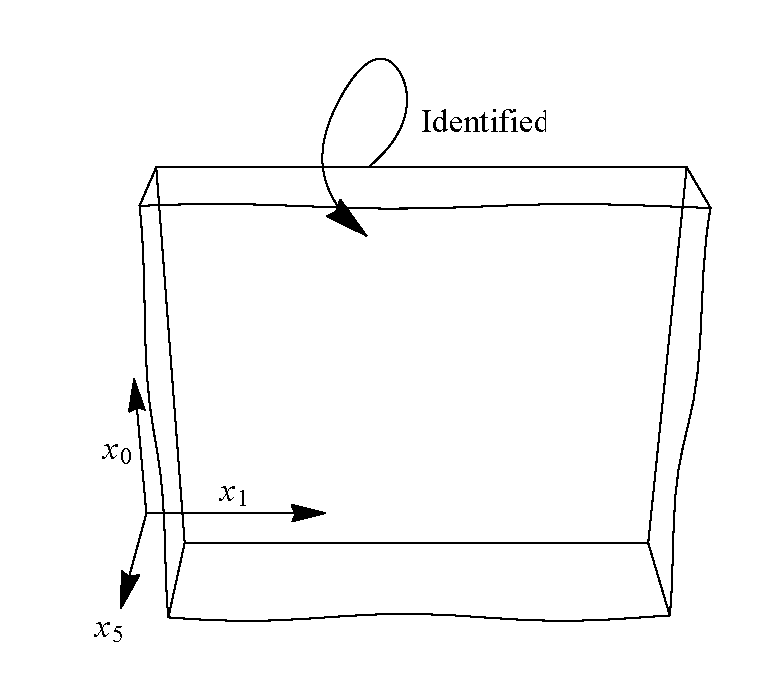
\includegraphics[scale=.52]{Graph11.pdf}}
\hfill
\subfloat[A function $\phi$ with two variables $x_0$ and $x_1$ on $\mathbb{R}^2$.]{\label{fig:Graph4}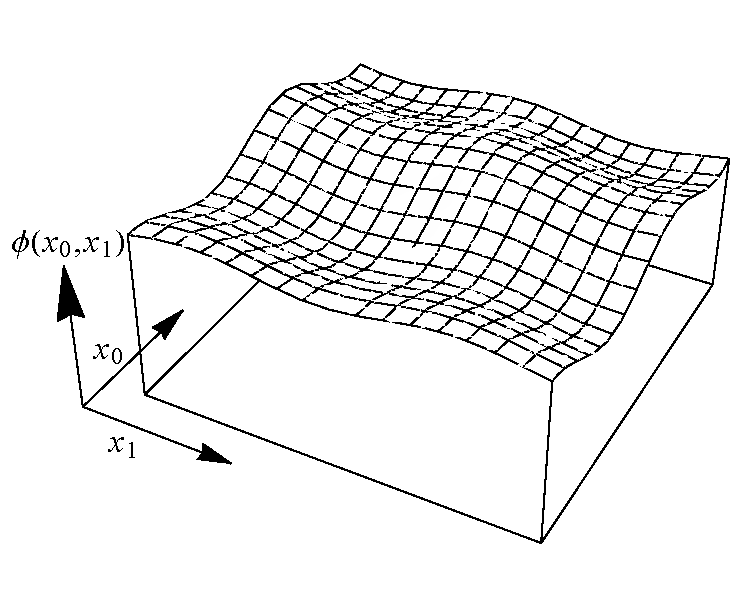
\includegraphics[scale=.5]{Graph12.pdf}}
\hspace{5mm}
\captionsetup{width=430pt}
\caption{The size of the fifth dimension $x_5$ can be seen as the value of the dilaton $\phi$.}
\label{fig:Graph3.png and Graph4.png}
\end{center}
\end{figure}

Experimentalists have never seen the dilaton. It seems this field is very hard to excite, for some unknown reason. If the Kaluza-Klein story is true, and the dilaton does exist, we are lead to conclude that the dilaton, and therefore the size of the fifth dimension, is always in its groundstate $\phi(x)=\phi_0$~\cite{Zee2013}.


\section{Causal-Set Technologies}
\label{sec:Causal-Set Technologies}
\subsection{Sprinkling}
\label{sec:Sprinkling}

We mentioned above, as expressed in equation~\ref{eq:Correspondence}, that a causal-set can be approximated by a continuous spacetime via the correspondence between the number of elements and the spacetime volume and between the partial order of the set and the causal structure. More precisely, a causal-set can be approximated by a spacetime if it can be faithfully embedded into a manifold. Embedding means that we assign spacetime coordinates to each element such that the partial order of the set agrees with the causal structure of the metric on that manifold~\cite{Bombelli1987}. Furthermore, once embedded into the spacetime, the elements need to be uniformly distributed. It has been proven that such a uniform distribution of elements leads to Lorentz invariance of the approximating spacetime, which is one of the key features of causal-set theory~\cite{Bombelli2006}. An embedding is called faithful if this last condition is met, but what exactly does a uniform distribution mean? To understand this, let us look at the concept of sprinkling.

Sprinkling refers to the process of placing causal-set elements into a spacetime in a random fashion, such that the number of elements $n$ per spacetime $V$ volume is given, in the limit, by the Poisson distribution:
\begin{equation}
\label{eq:Poisson distribution}
P(n)=\frac{(\rho V)^n e^{-\rho V}}{n!}
\end{equation}
Here, $\rho$ is the fundamental density which leads to every element taking up, on average, a Planck volume of spacetime. Once the elements are sprinkled into the manifold, the metric and the causal structure are used to infer the partial order between the elements.

The sprinkling process can be used in two ways. First, it can be used to define what we mean by a spacetime approximating a causal-set. A manifold with a metric can serve as an approximation for a causal-set if there is a high probability that that set could have come from a sprinkling into the manifold~\cite{Henson2009}. Sprinkling is not a fundamental process, it is not how causal-sets are actually created. Causal-sets are grown via a particular dynamical law. Although there are many ways to form a causal-set, not all of which faithfully embed into any manifold, it is assumed the growth-dynamics of causal-sets are such that the resulting set could have arisen from a sprinkling. Then, these causal-sets can be faithfully embedded into a realistic spacetime, such as our own.

At this moment, though, there is no fundamental dynamical law which can create arbitrary embeddable causal-sets from scratch. This is where the second use of a sprinkling comes in, namely to generate embeddable partial orders. Realistic causal-sets are often needed to do calculations and to test the hypotheses of the theory, and we, too, will need one to preform our Kaluza-Klein procedure. In particular, we will need to sprinkle into a five-dimensional spacetime where one dimension is compactified, as depicted in figure~\ref{fig:Graph3}. Sprinkling into a manifold of choice will result in a causal-set which, without any doubt, is embeddable into that same manifold.


\subsection{Dimension}
\label{sec:Dimension}

A causal-set does not inherently have a dimension\footnote{Once we fully know the laws of nature, including the growth-dynamics of causal-sets, would we be able adjust the dynamics so as to create an additional dimension?}. A causal-set is just a set of elements of which some are linked to each other. This can be visualised as a graph, and, as just explained, this graph may be embeddable into a manifold which does have a particular dimension. Without the requirement of a uniform distribution, most causal-sets will be embeddable into some manifold and we can define the Minkowski dimension of a causal-set as the dimension of the lowest dimensional manifold into which it can be embedded~\cite{Meyer1988}.

However, in the above definition, we did not require the embedding to be faithful, which is a necessity for causal-sets that hope to resemble a spacetime. Assuming we are dealing with a faithfully embeddable causal-set, there is a new dimension-estimator which may be defined. The first person to look into the concept of dimensions within a causal-set was Meyer. He introduced a measure which looks at the way volume scales in different dimensions~\cite{Meyer1988}. This would estimate what he named the Haussdorff dimension of a causal-set. Let us see what the relation between volume and dimension is exactly. It can be shown that, in continuous $d$-dimensional Minkowski spacetime, the volume of a diamond-shaped neighbourhood $A$ depends on the height of the diamond $T$ via:
\begin{equation}
\label{eq:Hausdorff dimension}
\text{volume}(A)=\frac{2 \text{ volume}(S^{d-2})}{d} \left(\frac{T}{2}\right)^d
\end{equation}
We already discussed the correspondence between volume and number expressed in equation~\ref{eq:Correspondence}a, that each causal-set element takes up, on average, a Planck volume of spacetime. As such, we can estimate the volume of diamond $A$ in a causal-set by simply counting the number of elements it contains. Then, if we know $T$, we can deduce the dimension of the set. The height of a spacetime-diamond in a causal-set can be estimated in different ways, one of which relies on looking for the longest chain from the bottom to the top of the diamond. We will discuss this below in section~\ref{sec:Space-Like Length}, as it is also important for measuring the space-like width of the diamond. By examining this method thoroughly, Meyer realised that chains of various lengths contain a lot of geometric information about the causal-set. He managed to formulate an expectation value $C_k$ for the number of $k$-length chains within a diamond and this eventually leads to the following expression which implicitly defines the Hausdorff dimension~\cite{Meyer1988}:
\begin{equation}
\label{eq:Hausdorff dimension2}
\frac{C_2}{C_1^2}=\frac{\Gamma(d+2)\Gamma(\frac{d+1}{2})}{4\Gamma(\frac{3(d+1)}{2})}
\end{equation}
This dimension-estimator has a interesting application to our Kaluza-Klein spacetime. The spacetime we are considering has five dimensions, of which one dimension is small and compactified. If the causal-diamond used to estimate the dimension is smaller than the circumference of the compactified circle, this estimator will have no idea about the compactification. As such, it is to be expected that the dimension is simply equal to five. However, as we increase the size of the diamond, the particular topology will become evident and the way the number of elements $C_1$ scales with volume will be different from the way the number of causally connected pairs $C_2$ scales. The estimator in equation~\ref{eq:Hausdorff dimension2} will then give a different result. Eventually, we expect the estimation to converge to four, if we look on scales much larger than the circumference of our compactified dimension. Indeed, this is what Meyer found in his simulations~\cite{Meyer1988}.

The Hausdorff dimension-estimator uses the volume-relation in equation~\ref{eq:Hausdorff dimension}, which is accurate for flat Minkowski space, to deduce the dimension of the set. As such, it is unable to deal appropriately with curvature. The estimator was recently updated by Roy et al.~\cite{Roy2012}. They used an expression for the volume of a diamond in a spacetime with first order curvature corrections~\cite{Myrheim1978}~\cite{Gibbons2007}. Similar to Meyer's approach, they worked out what the expected number of $k$-length chains $C_k$ would be in a causal-diamond with some curvature. As such, Roy et al. were able to formulate a new dimension-estimator capable of dealing with curved spacetimes. A side-effect of this was that they also found a way to extract curvature information from a causal-set. This will be discussed below, in section~\ref{sec:Ricci Scalar2}. In order to capture the effects of curvature, the dimension-estimation required more information than just the relation between $C_1$ and $C_2$. This can be achieved by including more types of chains, such as $C_3$ and $C_4$, into the calculation. The resulting expression for $d$, however, is very lengthy, so let us omit it.


\subsection{Coarse-Graining}
\label{sec:Coarse-Graining}

We have discussed the notion of approximating a causal-set by, and faithfully embedding it into, a manifold with a particular metric. However, there may be certain causal-sets which on the large scale seem realistic spacetimes, but on the small scale have wild fluctuations which inhibit it from being easily embedded into a manifold. To allow these types of sets to contribute to our quantum theory of gravity, Bombelli et al, who originally formalised causal-set theory, introduced the concept of coarse-graining. Under a coarse-graining, we randomly delete certain elements from our set~\cite{Bombelli1987}. More precisely, we can define a probability $p$ such that every element is retained with this probability and deleted with probability $1-p$. On a large scale, the new, coarse-grained causal-set $C'$ will be representative of our original $C$. In reality, however, it only preserves those features of $C$ which have a characteristic volume scale larger than $\frac{1}{p}$. As such, causal-sets which have wild fluctuations on a small scale will seem very dull after a coarse-graining. The process has washed out the small-scale structure.

This is particularly interesting for our five-dimensional Kaluza-Klein spacetime which has a special topology on the scale of the order $\phi_0$, the circumference of the compactified circle. Via a coarse-graining, small-scale features are removed. If we coarse-grain far enough, the fact that our original causal-set came from a sprinkling into a five-dimensional spacetime may be lost. The new, coarse-grained set would seem to only have a dimension equal to four~\cite{Meyer1988}. In section~\ref{sec:Ricci Scalar in Four Dimensions}, we will coarse-grain in a very particular way, to wash out all effects of the fifth dimension, and obtain the four-dimensional Ricci scalar.

In principle, there is an alternative to coarse-graining if we start off with a manifold. We could also sprinkle into a manifold with a density $\rho_E$ lower than the Planck density $\rho_P$. The difference between the effective density and the Planck density will, then, give the equivalent level of coarse-graining $p=\frac{\rho_E}{\rho_P}$. Either way, the small-scale structures are no longer visible and, similar to the dimension-estimation for a Kaluza-Klein spacetime described above, geometric quantities such as the Ricci scalar will presumably only take the four large dimensions into account.


\subsection{D'Alembertian}
\label{sec:D'Alembertian}

In the introduction, we discussed the approach by Johnston to define a scalar field on a causal-set via a path-integral. There is another way to look at the propagation of a scalar field on a causal-set and describing its dynamics requires the wave-operator, or d'Alembertian. If we assume the d'Alembertian $\square$ acts linearly on a scalar field $\psi$, it means, in the case of the discrete causal-set, that we are looking for a matrix $B_{xy}$ which approximates the action of the d'Alembertian on the field:
\begin{equation}
\label{eq:D'Alembertian}
\underset{l\rightarrow 0}{\text{lim}} \sum_y B_{xy} \psi_y=\square \psi(x)
\end{equation}
This matrix will be given by a particular expression which is dependent only on the causal-order of our set. One additional requirement of our matrix d'Alembertian $B$ is that it should only depend on elements in the causal past of what it is acting on. That is, it should be retarded in the sense that $B_{xy}=0$ whenever $x$ does not causally follow $y$.

In order to know how we should proceed to find an expression for $B$, let us look at the finite-difference method to see how derivatives are calculated in the discrete case. In particular, let us look at the backward difference and the second-order backward difference of a function:

\begin{subequations}
\label{eq:Finite difference}
\begin{gather}
f'(x)=\underset{\epsilon \rightarrow 0}{\text{lim}} \frac{\nabla_\epsilon[f](x)}{\epsilon}=\underset{\epsilon \rightarrow 0}{\text{lim}} \frac{f(x)-f(x-\epsilon)}{\epsilon}\\[1em]
f''(x)=\underset{\epsilon \rightarrow 0}{\text{lim}} \frac{\nabla^2_\epsilon[f](x)}{\epsilon^2}=\underset{\epsilon \rightarrow 0}{\text{lim}} \frac{f(x)-2 f(x-\epsilon)+f(x-2\epsilon)}{\epsilon^2}
\vspace{1mm}
\end{gather}
\end{subequations}

What we can learn from these equations is twofold. Firstly, values of the function at different steps away from $x$ are used. Secondly, the coefficients in front of these values seem to have alternating signs.

The first observation has a clear analogue in the case of causal-sets. When considering an element $x$, there are a number of elements which directly precede it. In fact, due to the non-compact nature of the Lorentz-group, there are an infinite amount of such elements. We may call this the first layer of $x$. There is also a second layer, one more 'step' away from $x$, which contains all the elements that precede $x$ and have exactly one other element in the interval in between them. These layers will be important in the definition of the discrete d'Alembertian.

The second observation of the alternating sign is also of importance as it turns out this helps tame the non-locality which is inherent in this approach to a d'Alembertian. This non-locality arises from the use of the nearest neighbours to $x$, those in the first layer, in the definition of our operator. Most of these neighbouring elements, in a sense, actually lie far away from $x$. They do, however, lie close to the past-lightcone of $x$ and that is the reason they are causally linked to $x$. If we want to reduce the impact of these 'far-away nearest neighbours', we need a mechanism which renders their effect on the d'Alembertian inert.

The original proposal for this approach to the discrete d'Alembertian was by Sorkin, who suggested summing over different layers of neighbours of $x$, with alternating sign~\cite{Sorkin2009}. It can be shown that this will, indeed, cancel out most of the non-locality. More precisely, he proposed summing over the first $3$ layers of $x$, which lead him to suggest the following discrete d'Alembertian for a two-dimensional causal-set:
\begin{equation}
\label{eq:D'Alembertian2}
B_2 \psi(x)=\frac{4}{l^2}\left(-\frac{1}{2}\psi(x)+\left(1\sum_{y\in L_1}-2\sum_{y\in L_2}+1\sum_{y\in L_3}\right)\psi(y)\right)
\end{equation}
Here, $L_i$ represents the $i$th layer of element $x$. Although the value of this d'Alembertian acting on $\psi$ will depend on the precise structure of the causal-set, it has been proven that, on average, it converges to the continuous d'Alembertian when the discreteness scale $l$ is taken to zero.

This approach has later been extended to a four-dimensional causal-set~\cite{Benincasa2010}. Finally, it was generalised to various dimensions for which it is easiest to write the matrix $B$ as~\cite{Dowker2013}:
\begin{equation}
\label{eq:D'Alembertian3}
B_d \psi(x)=\frac{1}{l^2}\left(\alpha_d \psi(x)+\beta_d \sum_{i=1}^{n_d} \gamma_{d i} \sum_{y\in L_i}\psi(y)\right)
\end{equation}
Here, the coefficients $\alpha$, $\beta$ and $\gamma_i$ are dependent on the dimension $d$ of the set. Furthermore, the number of layers $n$ to sum over is also different for different dimensions. However, the overall structure of the d'Alembertian is still the same in that we sum over layers of elements causally preceding $x$ with alternating signs.


\subsection{Ricci Scalar}
\label{sec:Ricci Scalar2}

Now that we have a d'Alembertian defined solely on the basis of the causal-set, you may wonder if it approximates the continuous wave operator for any type of causal-set, even those which would not be well approximated by a flat spacetime. It can be shown that, when there is curvature, the d'Alembertian actually approximates~\cite{Benincasa2010}:
\begin{equation}
\label{eq:Ricci scalar}
\underset{l\rightarrow 0}{\text{lim}} B_{d} \psi(y)=\left( \square-\frac{1}{2}R(x)\right) \psi(x)
\end{equation}
This means the definition of our discrete d'Alembertian can even deal with curvature, provided the curvature scale is much larger than the discreteness scale. It also means that there is an easy way to extract curvature information from any causal-set. Let us imagine there is a constant scalar field defined all over the causal-set with a value equal to $-2$. It was Benincasa et al. who realised that applying our matrix $B$ will then simply yield the Ricci scalar for that point~\cite{Benincasa2010}. In general, we may take our previous expression from equation~\ref{eq:D'Alembertian3} and define the discrete Ricci scalar as~\cite{Dowker2013}:
\begin{equation}
\label{eq:Ricci scalar2}
R_d (x)=-\frac{2}{l^2}\left(\alpha_d +\beta_d \sum_{i=1}^{n_d} \gamma_{d i} N_i(x)\right)
\end{equation}
Here, $N_i$ is simply the number of elements in the $i$th layer preceding $x$. Again, this expressions holds for various dimensions, each with different coefficients $\alpha$, $\beta$ and $\gamma_i$.

Interestingly, a slightly different expression for the Ricci scalar has also been formulated by Roy et al.~\cite{Roy2012}.
We have actually already seen much of this calculation in our discussion of the causal-set dimension in section~\ref{sec:Dimension}. Roy et al. had taken the original dimension-estimator by Meyer and extended it to deal with curvature. The dimension of a causal-set can be estimated by considering the abundance of $k$-length chains $C_k$. In a causal diamond with some curvature, the relative number of various length chains is different from the relative number in the case of flat spacetime. Therefore, by comparing the number of different chains, curvature information can be extracted. In particular, the expected number of $k$-length chains in a causal diamond of height $T$ is dependent on three coefficients, $T$, $R$ and on $R_{00}$, the time-time component of the Ricci tensor. As these are three unknowns, in order to extract the value of $R$, we need three different $C_k$'s. For example, one could choose to look at the total number of elements $C_1$, the number of causally connected pairs $C_2$ and the number of $3$-length chains $C_3$ within a causal-diamond. This can then give us an estimation of the curvature of that diamond. The resulting expression for $R$, however, is very lengthy, so let us omit it.


\subsection{Space-Like Length}
\label{sec:Space-Like Length}

In section~\ref{sec:Dimension} above, we mentioned that the height $T$ of a causal-diamond is related to the number of elements in the longest chain between the top and the bottom~\cite{Meyer1988}. Let us now make that more precise. The time-like length between any two points in continuous spacetime is the geodesic between those two points, where the geodesic is such that it maximises the proper time between the two events. Indeed, deviating from the geodesic would entail following a path closer to the lightcone, which has a shorter proper time. For a causal-set, a similar argument holds. Given that two elements $w$ and $z$ are causally related, there is a finite number of elements between them and we can easily identify the longest chain which links up these two points. We could simply define the number of elements in this chain as the distance between the two points, but it turns out there is still a dimension-dependent coefficient $m_d$ which needs to be included~\cite{Brightwell1991}. It can be shown that for a two-dimensional spacetime, this coefficient is equal to $2$. For higher dimensions, only bounds exist, but these still allow for a practical estimation of the time-like distance between two causal-set elements. In the limit of taking the discreteness-scale to zero, this measure converges to the distance between the two points in a continuous spacetime.

Because elements which are time-like separated are causally connected, it is quite easy to define a measure for the time-like distance in a causal-set. Extracting the space-like distance between two elements is more difficult however, as they are by definition causally unrelated. A first attempt was made by Brightwell et al., who realised that two space-like separated points can also be used to form a causal-diamond. The height of this diamond can then be estimated, which should be related to the space-like distance between the two points, as it would be in the continuum. More precisely, they proposed to measure the space-like distance between points $x$ and $y$ by looking for all points $w$ which lie in the causal-past of both $x$ and $y$ and by looking for all points $z$ which lie in their common causal-future. Calculating the time-like distance between all $w$'s and $z$'s and then selecting the smallest diamond between $x$, $y$, $w$ and $z$ should give a good estimate of the space-like distance between $x$ and $y$. The smallest diamond, in this case, is defined as the one which has the shortest time-like distance between top and bottom. This method fails, however, as there are random fluctuations in the distribution of the elements within the diamond. As such, it is always possible to Lorentz-boost to a particular frame where the diamond is exceptionally small and the time-like chain between $w$ and $z$ only contains $x$ and $y$, yielding a trivial distance equal to $2$.

Fortunately, the method was updated by Rideout et al. who understood that the requirement to select out the smallest diamond between the four points was causing the bias in the estimate~\cite{Rideout2009}. On average, the time-like distance between any $w$ and $z$ does give the correct estimate for the space-like distance between $x$ and $y$. It is merely the random fluctuations which means there are some frames in which the calculated length would not converge to the right number. The authors suggested averaging over the distances between all pairs of $w$'s and $z$'s which formed a smallest diamond. However, instead of defining the 'smallest diamond' to be the one for which the time-like distance between $w$ and $z$ was the smallest, they defined it in a different way. A smallest diamond between $x$, $y$, $w$ and $z$ is now taken such that $w$ and $z$ still lie in the causal-past or future of both $x$ and $y$, but with the restriction that there is no additional element between $x$ and $z$ nor between $y$ and $z$. They call a $z$ which satisfies this condition a $2$-link of $x$ and $y$. Indeed, it is obvious such an element is the 'closest' point which lies in the future of both $x$ and $y$. For every such $z$, there is a corresponding element $w$ which minimizes the time-like distance between them. Under this restriction the number of pairs of $w$'s and $z$'s to be considered is reduced and, when averaging over them, produces a good measure of the space-like distance between $x$ and $y$.

Now that we know how to determine the space-like distance between any two unrelated points, we immediately see a nice application of this measure in allowing us to determine the circumference of the compactified fifth dimension in our Kaluza-Klein spacetime. The details of this will be explained below, in section~\ref{sec:Dilaton2}. It turns out that, for this application, knowledge of the topology of the spacetime is required, in the form of the homotopy matrix.


\subsection{Covering Space}
\label{sec:Covering Space}

As the purpose of this paper is to combine Kaluza-Klein theory with causal-set theory, it is important to examine how the peculiar topology of a cylinder translates to the causal-set. A well known approach to dealing with cylinders is to 'unroll' them, i.e. to go to their covering space.
\vspace{-4mm}
\begin{figure}[h]
\begin{center}
\leavevmode
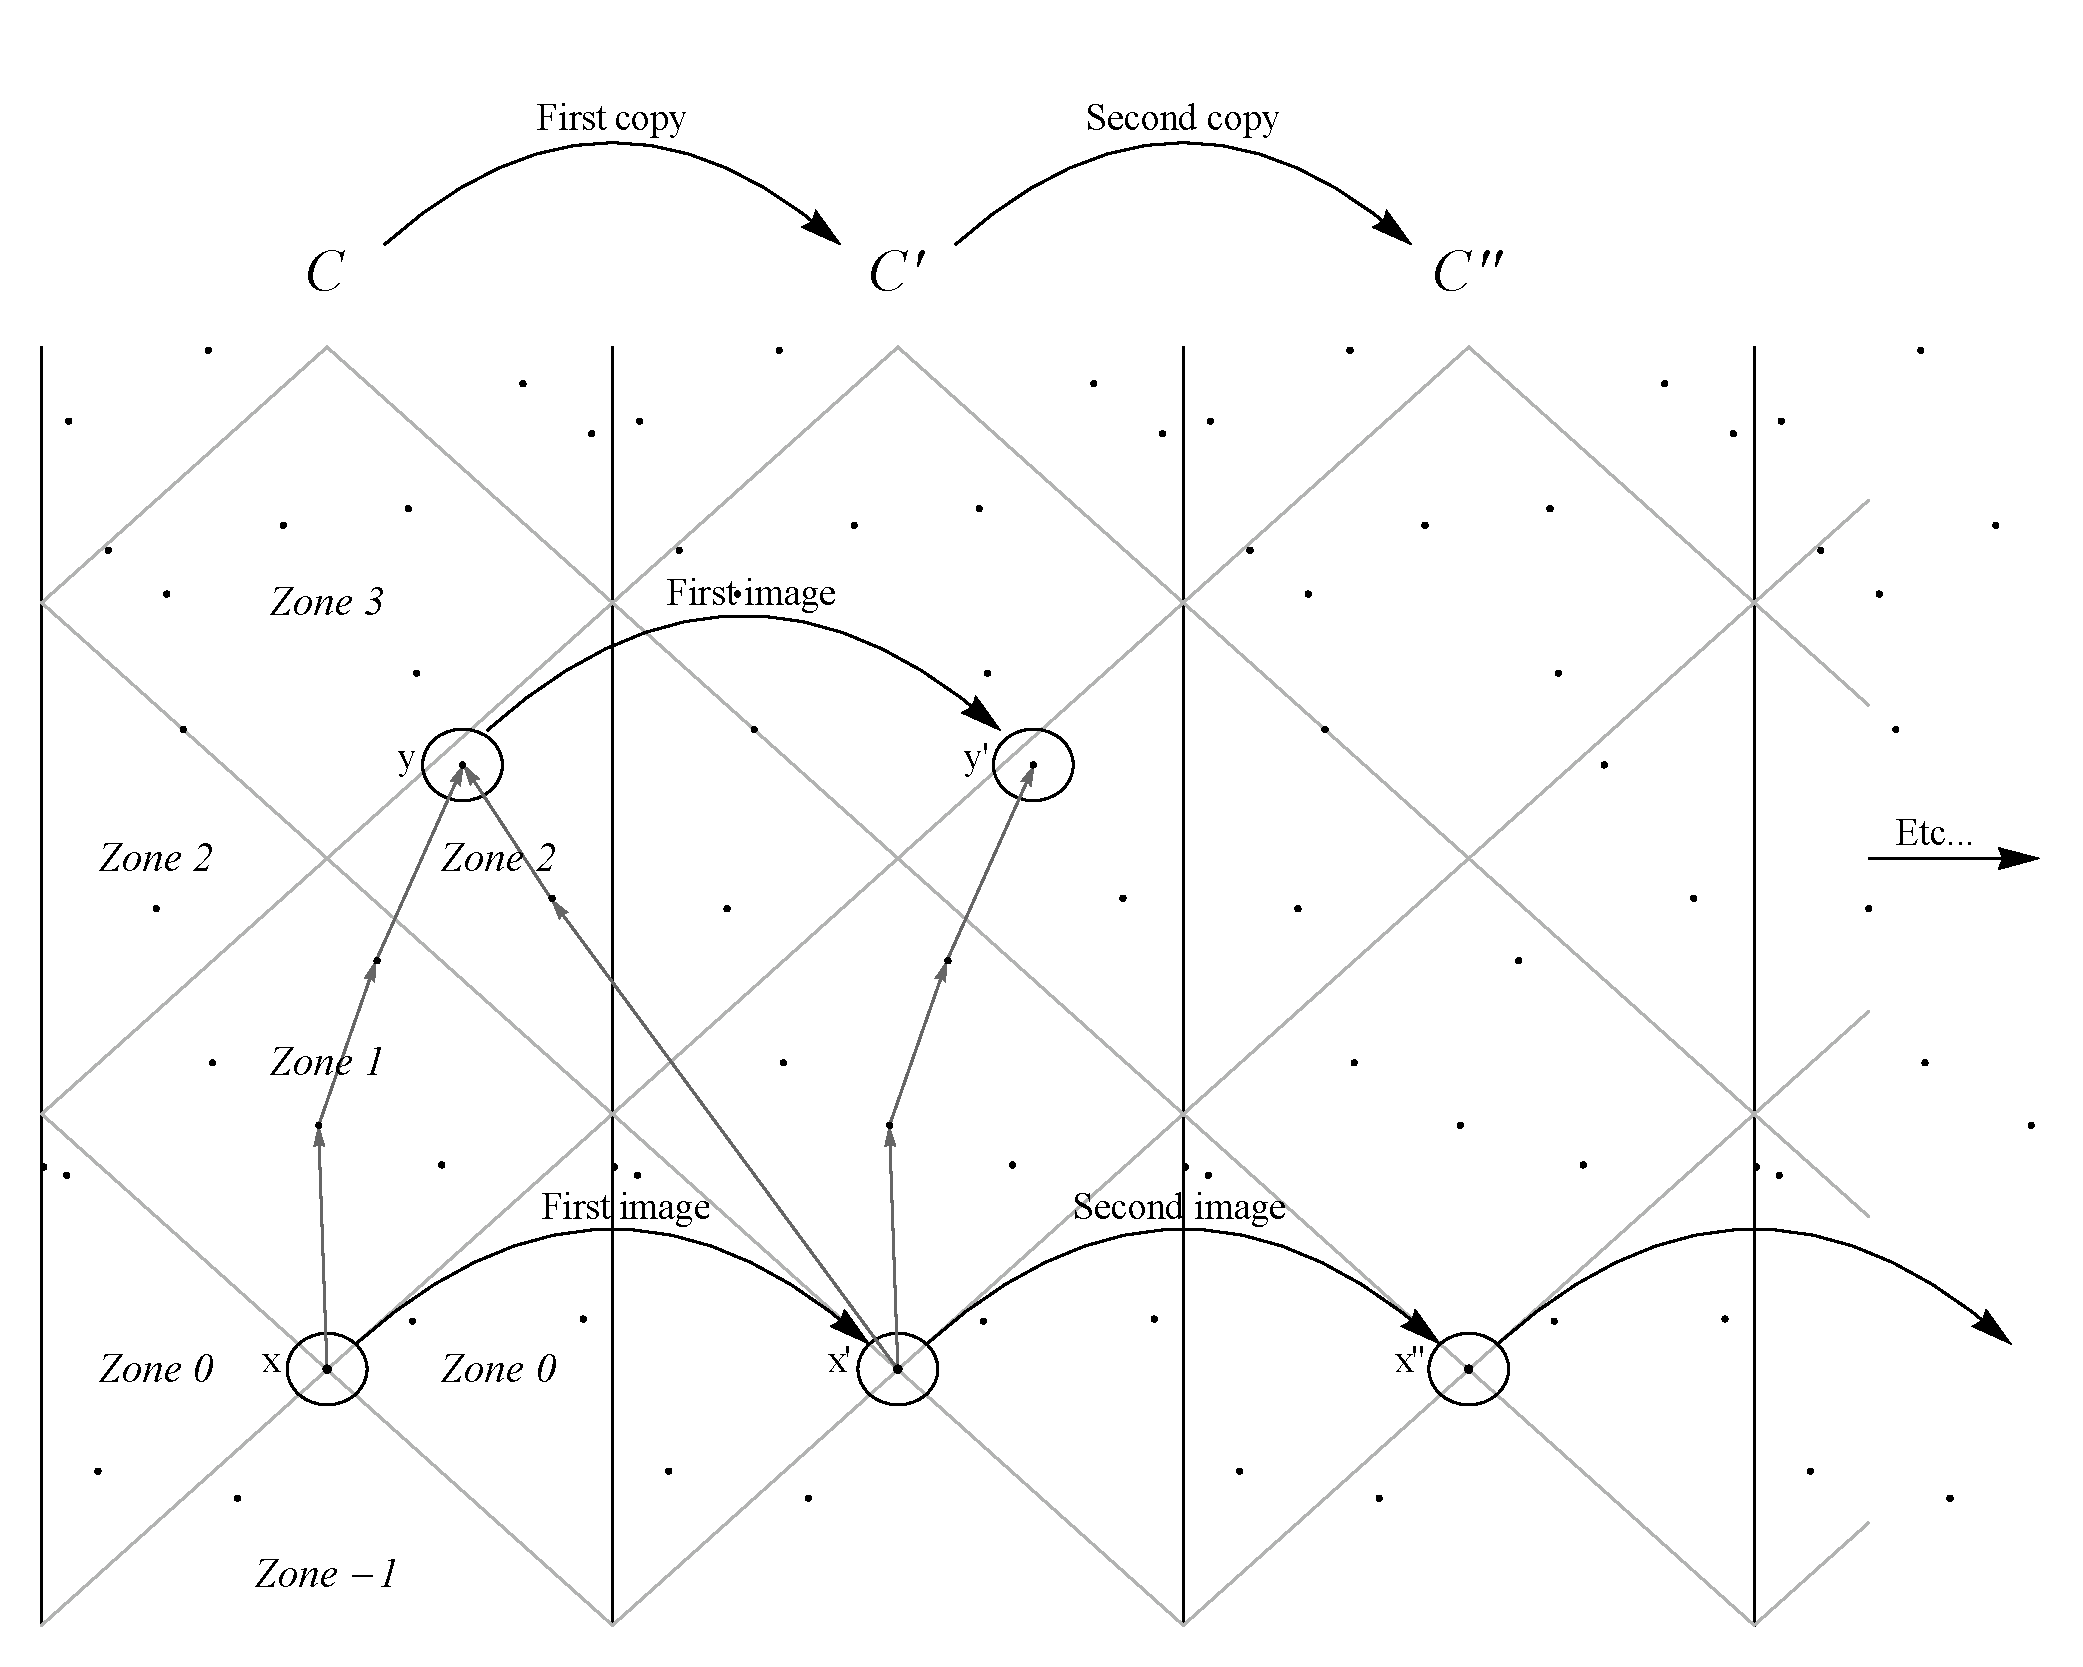
\includegraphics[scale=.44]{Graph14.pdf}
\caption{Unrolled cylindrical sprinkling depicting the various zones of element $x$.}
\label{fig:Graph14}
\end{center}
\end{figure}

 Let us examine the covering space of a cylindrical causal-set $C$ by sprinkling into a two-dimensional strip and then copying the points, in theory, an infinite number of times, naming the copies $C'$, $C''$ and so forth. Figure~\ref{fig:Graph14} depicts the point $x$, as well as its image $x'$ in the first copy of our sprinkling. As will become clear in section~\ref{sec:Dilaton2} below, it is the space-like distance between these two points which we are interested in. This length will give the value of the circumference of the compactified circle at that point. This length is the value of the dilaton.

The first person to investigate the covering space of a causal-set was Schmitzer. He was concerned with the Jonhston propagator, which we mentioned in section~\ref{sec:Matter Fields on Causal-Sets}, and how matter fields on a causal-set evolve when the spacetime has non-trivial topology, such as the cylinder~\cite{Schmitzer2010}.

In figure~\ref{fig:Graph14}, we can see various zones of element $x$. Zone $0$ are all elements which are space-like to $x$. Zone $1$ are the elements related to $x$, but not to its first image $x'$. Zone $2$ can be reached from $x$ as well as $x'$, but not from $x''$, and so on. These zones depict the number of equivalence classes of causal trajectories from this point $x$ to any other element. Let us call the matrix which lists in which zone a point is with respect to another point the homotopy\footnote{In~\cite{Schmitzer2010}, the homotopy matrix $H_C$ was referred to as $A_H$.} matrix $H_C$. Clearly, for the case in figure~\ref{fig:Graph14}, the value for $(H_{C})_{xy}$ is $2$. For point $y$, we can travel directly from $x$ upward to $y$. We can also travel from $x$ all the way around the cylinder and then reach $y$. This is the route from the image $x'$ to $y$. As such, element $y$ is in zone 2 with respect to $x$.

It is very easy to write down the zone-number for every element once we are in the covering space. From the unrolled sprinkling, we can determine the homotopy matrix. Likewise, once we have the homotopy matrix, it is possible to almost fully recreate the covering space. The trick, however, is to define things without mention of the sprinkling. The trick is to define things based solely on the causal-order. We are not allowed to use any information which is not fundamental to the partially ordered set.

Let us now try to recreate the homotopy matrix solely from the underlying causal-order. By staring long enough at figure~\ref{fig:Graph14}, an obvious way to classify elements into zones emerges. Let us define an element to be in zone 1, with respect to $x$, when it is causally related to $x$ but there exist an element space-like to it, which is also space-like to $x$. Zone $2$, then, are those elements causally related to $x$ for which all elements space-like to it are also causally related to $x$, but there exists an element space-like to it which is also space-like to an element from zone $1$. We can continue this step-by-step, moving upwards, to define all the zones, using solely the causal-order. We now have the homotopy matrix. This can be useful in various applications, one of which is to determine the space-like distance between $x$ and $x'$ and, therefore, to determine the value of the dilaton $\phi$.

Unfortunately, as was also clear to Schmitzer when he tried to recreate the homotopy matrix from the underlying causal-order, this procedure fails when the spacetime has a dimension larger than two~\cite{Schmitzer2010}. We will come back to this in section~\ref{sec:Dilaton2}.


\section{The Method}
\label{sec:The Method}
\subsection{Ricci Scalar in Five Dimensions}
\label{sec:Ricci Scalar in Five Dimensions}

The purpose of this paper is to introduce a method that allows us to define matter fields within a causal-set via a Kaluza-Klein approach. So far, we have reviewed a number of important technologies which have been developed in Kaluza-Klein theory and in causal-set theory. Each of these will serve a purpose in the following sections. Here, we start off by imagining a five-dimensional spacetime of which one dimension is compactified and small. We then sprinkle into this manifold and use the metric to infer the causal-order between the elements of the set. We then throw away the manifold and are left with a causal-set of which we know it can faithfully embed into our original spacetime.

After our discussion of the Ricci scalar in section~\ref{sec:Ricci Scalar2}, it is almost trivial to determine the curvature for each of the elements of the causal-set. We have seen two different ways to calculate this curvature, but for the following method, we only use the one Benincasa et al. originally proposed. For five dimensions, this is given by the following expression:
\begin{equation}
\label{eq:Ricci scalar in five dimensions}
R_5 (x)=\frac{1}{l^2 \Gamma (\frac{7}{5})}\left(\frac{\pi^2}{20\sqrt{2}}\right)^{\frac{2}{5}} \left(2-\frac{3}{4}N_1(x)+\frac{645}{64}N_2(x)-\frac{675}{32}N_3(x)+\frac{375}{32}N_4(x) \right)
\end{equation}
For completeness, let us remind ourselves that $N_i$ stands for the total number of elements in the $i$th layer of $x$, where we defined a layer to be all the elements which causally precede $x$ and have exactly $i-1$ other elements in the interval in between them. We see that it is, in principle, very easy to do this calculation for every single element in the causal-set, and that the answer only uses the information contained in our partial order.


\subsection{Dilaton}
\label{sec:Dilaton2}

The next step in our method will be to determine the value of the dilaton for every element. As we briefly mentioned above in section~\ref{sec:Space-Like Length}, we can use the measure for the space-like distance between two points to calculate the size of the fifth dimension. To do this, we need to unroll the compactified circle and go into the covering space of our causal-set.

Looking at the covering space depicted above in firgure~\ref{fig:Graph14}, it almost seems trivial to determine the space-like length between $x$ and $x'$. Let us see how to do it and then discuss why it fails. In section~\ref{sec:Space-Like Length}, we saw the approach by Rideout et al. which improves the original attempt by Brightwell et al., to define a measure which estimates the distance between two unrelated points. We will need to draw a causal-diamond between $x$ and $x'$ and then determine the height of this diamond. The procedure starts by looking for the $2$-links between $x$ and $x'$, i.e. all elements $z$ which lie in the future of both $x$ and $x'$ and are related to them without any other element in between. In principle, then, we would continue to search for a suitable element $w$ in the past of both $x$ and $x'$ and determine the time-like length between all $z$'s and their paired element $w$. As discussed in section~\ref{sec:Space-Like Length}, we simply average over all these pairs to obtain an estimate of the space-like distance between $x$ and its image. Obviously, in this case, $x$ and $x'$ are one and the same point. Therefore, every single element which is linked to $x$ satisfies the condition that it is a $2$-link between $x$ and $x'$. We need to be more precise about what types of $z$'s to consider.

Via the concept of zones, it becomes clear how to select the appropriate $2$-links. Elements which are causally related to both $x$ and $x'$ were considered to be in zone $2$, or higher. Therefore, to find a $z$ which satisfies the conditions set by Rideout et al. in their procedure, we now only look at $z$'s within zone $2$ , and pair them with $w$'s from zone $-2$. Determining the average time-like distance between all these pairs will give a good estimate of the width of the causal-diamond between $x$ and its image. Therefore, we finally have a measure\footnote{One more measure can be used in a two-dimensional cylinder, one which does not even require the homotopy matrix. We could calculate the distance between $x$ and every element space-like to it. The one with the largest space-like distance will be on the opposite side of the cylinder. As such, we simply take $2$ times this value as the circumference. However, this measure, too, fails in higher dimensions.} for the circumference of our cylinder.

In the above example, we used a two-dimensional cylinder. Our original Kaluza-Klein spacetime is five-dimensional, and this is where the method breaks down. In order to determine the zone-number of an element with respect to $x$, we made use of the fact that the number of elements space-like to $x$ is finite. In more dimensions, however, there are an infinite number of causally unrelated elements. We cannot make use of the step-by-step procedure to determine in which zone an element is. We cannot find the homotopy matrix based solely on the underlying causal-order. Although progress on recovering the topology of a causal-set is being made, how to solve this specific problem is still an open question~\cite{Major2007}.

Having failed at an attempt to calculate the circumference of our cylinder by looking at the space-like distance between $x$ and its image $x'$, we are lead to determine the circumference in a different manner. This brings us back the our earlier discussion of causal-set dimensions and the work of Meyer. We already briefly mentioned that the dimension of a Kaluza-Klein cylinder changes as we zoom-out and consider larger and larger causal-diamonds in our dimension-estimate. This suggests the estimator has some knowledge of the topology of the cylinder, and particularly, knows about the size of the cylinder. Indeed, Meyer himself already examined this relation and found that his method of comparing the relative abundance of $k$-length chains is powerful enough to formulate an expression for the circumference of the cylinder~\cite{Meyer1988}.
\begin{equation}
\label{eq:Circumference}
\frac{C_2}{C_1^2}=\frac{1}{2}-\frac{\phi}{4 T}-\frac{\phi^2}{24 T^2}
\end{equation}
As we want to allow for a dilaton which changes from point to point, we need to take into account a circumference of the compactified dimension which changes from point to point. Let us propose the following simple method to achieve this. For an element $x$, take any causal-diamond of height $T_0$ in its past such that $x$ causally proceeds all elements in the diamond. Determine the total number of elements $C_1$ in this diamond, as well as the number of $2$-length chains $C_2$, and use equation~\ref{eq:Circumference} with $T=T_0$ to obtain the circumference of the cylinder, or the value of the dilaton $\phi$, at $x$. 
\begin{equation}
\label{eq:Circumference2}
\phi(x)=\sqrt{21-32 \frac{C_2(x)}{C_1(x)^2}}T_0-3 T_0
\end{equation}
What size causal-diamond to use depends a bit on the situation. For a good estimate, $T_0$ must be substantially larger than the size of the dilaton. This is because the diamond needs to wrap around the cylinder to be able to know about the topology. Like with the dimension-estimator, if the diamond is too small, it would not notice the compactification. At the same time, $T_0$ need to be substantially smaller than the scale at which the dilaton changes value. This is because the estimate for $\phi$ uses a diamond which stretches into the past of element $x$, and if $\phi$ rapidly changes value, the estimate for $x$ will be biased by what happened in its recent past.


\subsection{Ricci Scalar in Four Dimensions}
\label{sec:Ricci Scalar in Four Dimensions}

We have mentioned several times that the small-scale structure of a causal-set will go unnoticed when larger causal-diamonds are used. This occurred, for example, when estimating the Hausdorff dimension of a cylinder~\cite{Meyer1988}. Coarse-graining provides another way to wash out the effects of the small-scale structures. In section~\ref{sec:Coarse-Graining}, we discussed that coarse-graining using a probability $p$ will produce a new causal-set which only preserves those features with a characteristic volume scale larger than $\frac{1}{p}$. If we take our five-dimensional Kaluza-Klein spacetime, and we coarse-grain far enough, the entire fifth dimension will simply fade away. We are then left with a four-dimensional hypersurface, a four-dimensional causal-set.

To achieve this, we need to coarse-grain in a very particular way. We need to coarse-grain at a level equal to the size of the fifth dimension. This size, represented by the value of the dilaton, is not necessarily the same everywhere. If we want the fifth dimension to collapse into a single point, such that only four dimensions remain, let us coarse-grain at a level equal to $\phi(x)$. As every element in our set has its own value for $\phi$, determined above in section~\ref{sec:Dilaton2}, the probability that an element is deleted is different for all elements. We retain\footnote{In practice, a coarse-graining probability of $\frac{1}{\phi}$ may be too harsh. Using $\frac{10}{\phi}$ or $\frac{100}{\phi}$ may be better.} this element in our coarse-grained set with probability $\frac{1}{\phi}$ and delete it with probability $1-\frac{1}{\phi}$, where $\phi$ is expressed as the dimensionless number of elements the compactified circle is wide at that point.

Now we are left with a causal-set which is representative of our original causal-set while only preserving those features which have a characteristic volume scale larger than $\phi$. This means the entire fifth dimension has been washed out, leaving a causal-set which faithfully embeds into a spacetime with four non-compactified dimensions. This allows us to determine the value of the lower-dimensional Ricci scalar. For every element in our original causal-set, we take the coarse-grained set and, if the element we are considering is not there, we add it back in. We then simply use the procedure outlined in section~\ref{sec:Ricci Scalar2} above, using the coefficients for a four-dimensional spacetime, to obtain the value for the curvature at that point.
\begin{equation}
\label{eq:Ricci scalar in four dimensions}
R_4 (x)=\frac{1}{l^2}\sqrt{\frac{2}{3}} \left(4-4 N'_1(x)+36 N'_2(x)-64 N'_3(x)+32 N'_4(x) \right)
\end{equation}
Here, $N'_i$ stands for the number of elements in the $i$th layer of element $x$ in the coarse-grained set.


\subsection{Electromagnetic Field Strength}
\label{sec:Electromagnetic Field Strength}

We now have a value for the five-dimensional Ricci scalar for every element of our Kaluza-Klein causal-set. We also have the value of the dilaton for every one of these elements. Furthermore, we just saw how to assign a value for the four-dimension Ricci scalar to every single element. Finally, we are in a position to talk about the electromagnetic field strength $F_{\mu \nu } F^{\mu \nu}$, the magnitude of the gauge field which results from the Kaluza-Klein process. In section~\ref{sec:Ricci Scalar}, we saw that the five-dimensional Ricci scalar of a continuous spacetime with one dimension compactified splits into three distinct parts: one part is the four-dimensional Ricci scalar, one part represents a gauge field and one part referring to a scalar field:
\begin{equation}
\label{eq:Four-dimensional Ricci scalar}
\tilde{R}=R+\frac{1}{4} \phi^2 F_{\mu \nu } F^{\mu \nu}+\frac{\square \phi}{\phi}
\end{equation}
In the case of the causal-set, we have expressions for three of the four unknowns in this equation. We can, therefore, solve for the electromagnetic field strength and express it using solely the causal-order.
\begin{equation}
\label{eq:Four-dimensional Ricci scalar}
F_{\mu \nu }(x) F^{\mu \nu}(x)=\frac{4}{\phi(x)^2} \left( R_5(x)-R_4(x)-\frac{B_4 \phi(x)}{\phi(x)} \right)
\end{equation}
Each of these terms, including the d'Alembertian $B_4$, only makes reference to the causal-order. We have shown that a causal-set, a locally finite partially ordered set, through geometry alone, can represent a spacetime in which matter fields propagate.


\section{Conclusion}
\label{sec:Conclusion}
\subsection{Size of the Extra Dimension}
\label{sec:Size of the Extra Dimension}

In this paper, we examined a method to combine Kaluza-Klein theory with causal-set theory. In order to fully understand the method, we had to review several technologies within both theories. Sprinkling and coarse-graining are such technlogies, and we discussed that a causal-set is approximated by a spacetime if it could have arisen from a sprinkling into that spacetime. Furthermore, it would then support features of that spacetime which are larger than a characteristic scale related to the density of points per spacetime volume. This leads us to wonder how many points are sprinkled into the fifth dimension. How many points is the compactified dimension wide? What density is needed so that the causal-set can capture the geometrical structure necessary in Kaluza-Klein theory?

The compactified dimension needs to contain a relatively large amount of causal-set elements. If the amount is too small, the small-scale features would not be visible, or more precisely, would simply not be there. This is the reason the coarse-graining in section~\ref{sec:Ricci Scalar in Four Dimensions} worked. By coarse-graining, we reduced the number of elements to the point where the fifth dimension completely disappeared. To be able to support a gauge field and a scalar field, the fifth dimension needs to have a minimum 'resolution' in terms of the density of points.

From this minimum density, we can argue that the fifth dimension also has a minimum size. For the sake of argument, let us assume the circumference of the compactified dimension needs to be\footnote{The precise number is irrelevant, the gist of the argument holds.} at least $10^3$ individual points wide. If the discreteness scale is indeed around the Planck scale, this means the fifth dimension is about $10^{-33}$ m in size. It cannot be much smaller, and certainly not around the Planck scale itself, as theorists often assume, as that would mean the circle contains less points. With too few points, it would not be able to support the geometric structure which represents our gauge field and scalar field.

Current experiments put an upper-bound on the size of the additional dimension. In particular, it cannot be larger than $10^{-18}$ m, otherwise we would have noticed it~\cite{Overduin1997}. There is also a theoretical argument which puts an upper-bound on the size. One of the main predictions of causal-set theory concerns the value of the cosmological constant. The argument goes that there is a Heisenberg uncertainty relation between the variance of the volume of spacetime and the variance of Lambda. As there is a correspondence between number and volume, mediated by a Poisson process, the variance of our spacetime volume is proportional to the squareroot of the number of causal-set elements. We can estimate the number of elements by considering the discreteness scale, which, in turn, is set by considering black hole entropy. This is where the gravitational constant $G$ comes in. If there is indeed an additional, or even several additional dimensions, the true gravitational constant $\tilde{G}$ would lead to a different discreteness scale, and thereby a different estimate for Lambda~\cite{Sorkin2005}. Experiments have confirmed that Lambda is around the value predicted by causal-set theory in a four dimensional spacetime. If there are more dimensions, these cannot be too big. Only small extra dimensions lead to a prediction of Lambda which falls in the experimentally confirmed range. However, as the prediction for Lambda is only for its variance, no precise number can be placed on the maximum size of any additional dimension. Large extra dimensions simply make the predicted value less likely.


\subsection{Limitations of the Method}
\label{sec:Limitations of the Method}

The coarse-graining which we performed in section~\ref{sec:Ricci Scalar in Four Dimensions} in order to arrive at an expression for the Ricci scalar in four dimensions has a harmful side-effect. With the coarse-graining, we hoped to collapse the fifth dimension to a point such that only four dimensions remained. This collapse, however, can happen at different places, leading to an increase in the variance of the four-dimensional Ricci scalar estimate. In particular, the variance of this estimate is increased by an amount of the order of the size of the additional dimension which we tried to coarse-grain away. Let us see how that works.

\begin{figure}[h]
\begin{center}
\leavevmode
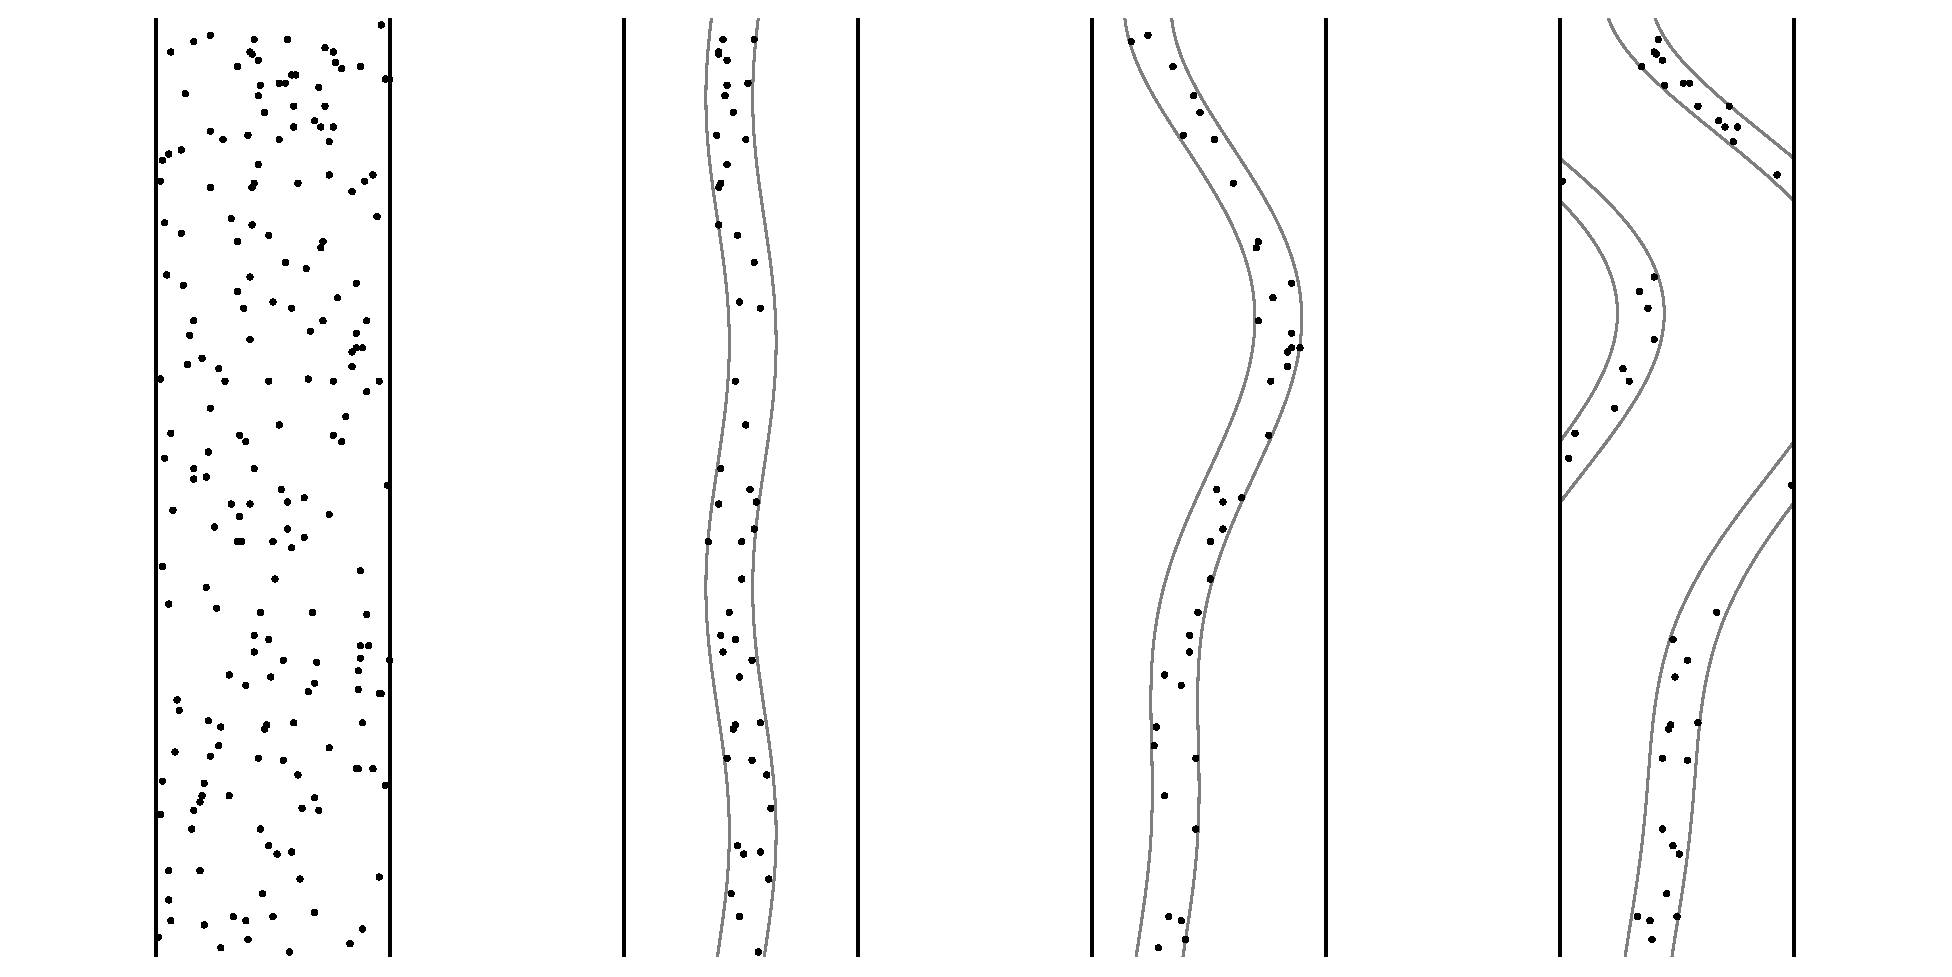
\includegraphics[scale=.44]{Graph13.pdf}
\caption{After coarse-graining, the remaining four dimensions can show additional curvature. Coarse-graining increases the variance in the estimate of the Ricci scalar.}
\label{fig:Graph13}
\end{center}
\end{figure}

Figure~\ref{fig:Graph13} shows the original strip into which we sprinkled where the two edges are identified. Under a coarse-graining, we hope points will be deleted so as to leave a nice, straight four-dimensional hypersurface for which we can determine the Ricci scalar. In reality, however, there is a chance the points do not lie on a straight line and, in a spacetime with a dimension higher than two, this can result in additional curvature. This effect is not limited by the size of the compactified dimensions, but it is expected higher fluctuations become ever less likely. If the additional variance in the curvature is of the same order as the curvature within the four dimensions, this can seriously undermine the method. In order to avoid this problem in our method, we might need to coarse-grain multiple times and average over the various new causal-sets to obtain a nice value for the four-dimensional Ricci scalar.

Another form of averaging over fluctuations was discussed by Sorkin in his work on the d'Alembertian~\cite{Sorkin2009}. The reason we did not discuss that earlier is that such an averaging is not fundamental. It is merely a procedure to check whether the discrete version converges to the continuous one in the limit. In fact, the calculation for the discrete d'Alembertian, which is also of essence in the culculation of the Ricci scalar, gives an expectation value which has been proven to converge to the continuous d'Alembertian. For an individual element, however, the value may be very different from the expectation value. Sorkin suggested taking patches of elements and averaging over them to obtain a measure of the d'Alembertian which does not have such a high variance in the estimate. This step can be included in our method too, as a way to dampen fluctuations and to test whether the method leads to the correct continuous expression in the limit.

We briefly mentioned in section~\ref{sec:Ricci Scalar} that we have been working in the Jordan frame. There is some debate whether it would be better to conformally rescale the metric to the Einstein frame~\cite{Overduin1997}. We did not concern ourselves with that debate here, and continued to work in the Jordan frame, as it proved easier to translate the continuous action to the discrete action in this frame. This is because in the Einstein fame, we are forced to include terms to the four-dimensional Ricci scalar like $\partial^\alpha \phi \partial_\alpha \phi$ for which there is currently no casual-set analogue. If it turns out the Einstein frame is indeed theoretically superior to the Jordan frame, we need to reconsider this part of our method.

In section~\ref{sec:Dilaton2}, we discussed the failure of the space-like length estimator to provide us with information about the dilaton. In order to determine the value of the dilaton at point $x$, we need to know the size of the circumference of the compactified dimension at that point. This means estimating the space-like distance between point $x$ and that exact same point, one tour around the circle. In the covering space, this calculation is easy once we have the homotopy matrix. But there is currently no method to determine the homotopy matrix for causal-sets with a dimension higher than two. Hopefully in the future this limitation will be removed.

Lastly, there are some theoretical problems with Kaluza-Klein theory in general~\cite{Zee2013}. One open question is how the fifth dimension becomes compactified in the first place. There have been many proposals for mechanisms which can lead to compactification of a dimension, but none so far have been very compelling. Another problem with standard Kaluza-Klein theory is that of parity violation. Parity violation in the weak interaction has been well established, but a simple Kaluza-Klein-like model, which views the weak interaction as a result of higher dimensional compactified spheres, can never lead to such a symmetry breaking.


\subsection{Updating the Method}
\label{sec:Updating the Method}

The method that was proposed in this paper to define matter fields in a four-dimensional causal-set relies on various technologies. Some of these technologies, such as calculating the Ricci scalar, can be achieved via two different procedures. In section~\ref{sec:Ricci Scalar2}, we discussed the proposal by Benincasa et al. to obtain the Ricci scalar by applying the discrete d'Alembertian to a constant field with a value equal to $-2$. The way the d'Alembertian is defined means that this procedure extracts curvature information by comparing $k$-element intervals, i.e. the various layers of element $x$~\cite{Benincasa2010}. Roy et al. found a very different method of extracting curvature information by adapting the dimension-estimator. This procedure compares the relative abundance of $k$-length chains within a causal-diamond. This suggests there is a relation between these two seemingly different causal-set entities, the intervals and the chains~\cite{Roy2012}. Moreover, it suggests we are able to pick and choose which procedure is more suitable for our method. If, in the future, there are arguments which clearly favour one of the two approaches, or if a third estimator of the Ricci scalar is defined, we can simply update our method without needing to change much to the overall outline.

In section~\ref{sec:Dilaton2}, we saw not only how the space-like length estimator failed in our particular case, but also that there was an additional method to determine the size of the compactified dimension. This second method was again an adaptation of the dimension-estimator. By comparing the relative abundance of $k$-length chains, a value for the dilaton could be given. Once more, we are lead to conclude that the method can easily be updated to include different, newer estimators and technologies. In the end, computer simulations may be needed to show which combination of procedures gives the best results.

Whatever causal-set technologies will be discovered in the future, this paper has provided a working method to define the four-dimensional Ricci scalar, the action of a gauge field and a scalar field. Further research and computer simulations are needed to show that this method is on the right track. Whether this will enable us to define an action leading to a quantum dynamics for causal-sets remains to be seen. At the very least, this paper hopes to have shown that Kaluza-Klein theory can, in principle, be combined with the causal-set approach to quantum gravity, and that vastly different entities such as space, time, matter and geometry can emerge solely from a partially ordered set.


\newpage

\phantomsection
\label{sec:Bibliography}
\addcontentsline{toc}{section}{Bibliography}
\renewcommand{\refname}{Bibliography}
\bibliographystyle{plain}
\bibliography{Bibliography}

\newpage

\appendix

\section{An Additional, Indirect Method}
\label{sec:An Additional, Indirect Method}
\subsection{Obtaining the Metric}
\label{sec:Obtaining the Metric}

The method suggested in this paper to combine Kaluza-Klein theory with causal-set theory follows the route of defining the Ricci scalar in terms of causal-set quantities. This is because the five-dimensional Ricci scalar breaks into three parts via the Kaluza-Klein procedure and for each of these parts a causal-set analogue can easily be defined. There is another method, however, to combine the two approaches. This goes through defining a metric in terms of causal-set quantities. Once the metric is known, the standard procedure of splitting the five-dimensional tensor into the four-dimensional metric, a gauge field and a scalar field, becomes a trivial matter.

Within causal-set theory, there have been many attempts to obtain geometric information solely from the underlying partial order. All of these attempts work towards proving that any relevant continuous quantity, such as the metric, can be obtained from the causal-set. One paper by Major et al. looks at thickened anti-chains~\cite{Major2007}. Anti-chains are a bunch of unrelated elements which can be thickened by including several layers of elements causally related to each of the elements in the original bunch. In a causal-set, they are the closest analogue to a Cauchy hypersurface. From the thickened anti-chains, topological information can be extracted and this is then used to recover the homology of a globally hyperbolic spacetime from the causal-set.

Rideout et al. also add to the discussion by speculating how the metric can be obtained. They suggest recovering the tangent space for an element $x$ by examining its closest neighbours~\cite{Rideout2009}. The tangent space is a vector space and so requires knowledge of the angles between each of these neighbours. Via their method of determining space-like distances, and the method of determining time-like distance, some information about angles may be available.

Certainly the most promising approach to obtaining the metric is by Henson. He defines a simple algorithm which produces coordinates for the causal-set elements~\cite{Henson2006}. In section~\ref{sec:Sprinkling}, we discussed that sprinkling is not a fundamental process but that it is an easy way of producing a realistic causal-set. Once points are sprinkled and the causal-relations are inferred, the coordinates for each of the points are thrown away, leaving only the partial order. The method by Henson can retrieve these coordinates, solely from the underlying relations. In fact, in simulations, it was shown the causal-relations of the elements in their new coordinates agree with the original causal-relations obtained after the sprinkling to about $99.66\%$. While this method assumes the spacetime is flat, and is therefore not very useful for obtaining the metric, the method may in the future be extended to deal with curved spacetimes. In section~\ref{sec:Obtaining the Metric by Graph-Drawing} of this appendix, a similar method is proposed which may do just that.

The algorithm by Henson works as follows. For a causal-diamond of $N$ elements, the coordinates of the bottom-most element can be defined as $(0,0)$, while the top-most element is placed at $(\sqrt{N},\sqrt{N})$. For a third element, the time-like distance to the top-element and that to the bottom-element is calculated. This is used to place it at an appropriate position within the causal-diamond. The same procedure is used for the next element, and, if possible, the time-like distance to the third element is used to take care of any remaining degrees of freedom. Step-by-step, all elements within the causal-diamond are given coordinates. Finally, the new causal-relations between the elements are obtained from these coordinates. The points are then moved by small distances in order to minimise the discrepancy between these new causal-relations and the original ones. For relatively small causal-sets, this algorithm provides a very simple way to lay out the graph of interconnected elements. Works such as these may eventually be used to obtain the metric for any manifold-like causal-set.


\subsection{Standard Procedure}
\label{sec:Standard Procedure}

In this paper, we saw that most of the causal-set analogues of geometric quantities, such as the dimension-estimator, made use of the information contained in $k$-length chains, the number of elements in a layer $N_i$ and the height $T$ of a causal diamond. As such, we may assume that, if an approach to obtaining the metric is found, the resulting tensor will be a function of these quantities.
\begin{equation}
\label{eq:Metric as a function}
\tilde{g}_{MN}(x)=f_{MN}(C_k(x, T), N_i(x), T)
\end{equation}
For a causal-set which faithfully embeds into a five-dimensional spacetime with one dimension compactified, we can then follow the standard Kaluza-Klein procedure to obtain values for the four-dimensional metric, the gauge field and the scalar field~\cite{Bailin1987}. In particular, following equation~\ref{eq:Metric}, we define these as follows:
\begin{subequations}
\label{eq:Indirect Kaluza-Klein}
\begin{gather}
g_{\mu\nu}(x)=f_{\mu\nu}(C_k, N_i, T)-\frac{f_{\mu 5}(C_k, N_i, T)f_{5 \nu}(C_k, N_i, T)}{f_{55}^2(C_k, N_i, T)} \\
A_\mu(x)=\frac{f_{\mu 5}(C_k, N_i, T)}{f_{55}^2(C_k, N_i, T)} \\
\phi(x)=f_{55}(C_k, N_i, T)
\end{gather}
\end{subequations}
These values can be used to construct the four-dimensional Ricci scalar and the electromagnetic field strength, such that a comparison with the main method of this paper can be made.


\section{Obtaining the Metric by Graph-Drawing}
\label{sec:Obtaining the Metric by Graph-Drawing}
\subsection{Extract the Coordinates}
\label{sec:Extract the Coordinates}

In this section, we will look at a novel proposal to construct the metric out of a causal-set. In particular, we will examine how the relations between causal-set elements can be used to place them in a hyperspace. Remember that there is a correspondence between the number of elements and the spacetime volume, as expressed earlier in equation~\ref{eq:Correspondence}~\cite{Bombelli1987}. If there is a region which has a larger density of points, this region has a larger volume. This is how curvature occurs in the causal-set. This instance would be similar to the surface of sphere, where the inner shells have a higher volume relative to the outer shells, corresponding to a positive curvature. But what is the conversion rate between the number of elements and volume? Several arguments exist which mostly point to the same answer. For example, when examining the entropy of a black hole horizon, it seems there is one bit of entropy per plaquette of size $8\pi G\hbar$. This leads to a discreteness scale $l=\sqrt{8\pi G\hbar}$ around the Planck length~\cite{Sorkin2003}. Every element seems to want to occupy the same amount of spacetime.

This means that there are two forces which determine the relative position of causal-set elements. First of all, there is a force which tells each element to 'take up' around a Planck volume of spacetime. You can visualize this as a set of elements which grow like soap-bubbles until they are all around the same size. Each bubble touches its surrounding bubbles such that the whole set makes a surface in the hyperspace.

The second force which acts between the elements constrains bubbles which are linked to each other. The step from one element to the next should also be about a Planck length long. Whenever two elements are causally linked, they are constrained to be around this distance away from each other within the hyperspace.

Given these two forces, we can try to think of an algorithm which is able to give coordinates to each of the causal-set elements within the hyperspace. The idea is quite similar to Henson's algorithm discussed in section~\ref{sec:Obtaining the Metric} above. He proposed using the time-like distance to the top of a causal-diamond and the distance to the bottom to determine and element's relative position~\cite{Henson2006}. By looking at the repulsive forces of the growing soap-bubble, while constraining them by Planck-sized links, a similar effect occurs.

Let us now imagine an algorithm which starts off by placing the causal-set elements in a random position. For each element, it determines the distance to every other element. It then calculates the repulsive force $f_r(i, j)$ acting on it due to all the other elements trying to take up a Planck volume. It also looks at all the elements which are linked to it and calculates the attractive force $f_a(i, j)$ running only through those links. 
\begin{subequations}
\label{eq:Forces}
\begin{align}
f_r(i, j) & = -\frac{K^2}{\parallel x_i - x_j\parallel} & \hspace{-24mm} i \neq j \hspace{8mm} i, j \in G \\
f_a(i, j) & = \frac{\parallel x_i - x_j\parallel^2}{K} & i \leftrightarrow j
\end{align}
\end{subequations}
These forces can then be used to displace the element slightly, in the direction of the total force. The process is repeated until a steady-state is reached. In principle, the two forces acting between all elements give the causal-set a particular energy. The energy is minimised when the elements are in the 'right' position. This is what the algorithm does.


Although we are looking for a method to deal with causal-set elements in a Lorentzian manifold, the algorithm just described already exists for Euclidean and Riemannian manifolds. In fact, there is a large body of work done on so called 'graph-drawing algorithms', and in particular on 'spring embedders' where links are replaced by springs to form a mechanical system~\cite{Kobourov2007}. The spring forces on the elements move the system to a minimal energy state.

In Riemannian manifolds, the algorithm is slightly more complicated in that distances are defined in terms of geodesics. In this case, the metric of the hyperspace into which you are embedding the elements is needed. More precisely, the algorithm computes the forces acting on an element $n$ at position $x$ in its tangent space $T_xM$ where $\tau_x$ is the map from the manifold $M$ to this tangent space~\cite{Kobourov2002}. The pseudo-code for this algorithm is the following:
\vspace{3mm}
\begin{equation}
\label{eq:Riemannian algorithm}
\begin{array}{l}
\texttt{generate initial layout}(G)\\
\texttt{while not done do}\\
\hspace{5mm} \texttt{foreach } n \in G \text{ do}\\
\hspace{10mm} x := \texttt{position}[n]\\
\hspace{10mm} G' := \tau_x(G)\\
\hspace{10mm} x' := \texttt{force directed placement}(n, G')\\
\hspace{10mm} \texttt{position}[n] :=\tau_x^{-1}(x')\\
\hspace{5mm} \texttt{end}\\
\texttt{end}
\end{array}
\end{equation}

In theory, the Riemannian metric can be extended to a pseudo-Riemannian one, such as for Minkowski space. Determining the map $\tau_x$ to the tangent space is the hardest step.

These algorithms have also been translated to $Mathematica$ code~\cite{Hu2005}. There are two different algorithms. One has both repulsive and attractive forces running through every link, such that each link has an optimal Planck-sized length. The other has its repulsive force between every element such that they all take up about a Planck volume. For our causal-sets, a combination of these two algorithms may be most appropriate.

In order to see if these procedures are capable of dealing with flat space, curved space and compactified space, let us examine the algorithms for a sprinkling into a Euclidean geometry. It is then suggested that generalising the codes to deal with a Lorentzian manifold will provide one way of obtaining the metric for realistic causal-sets.

\begin{figure}[h]
\begin{center}
\subfloat[Flat sprinkling]{\label{fig:Graph1}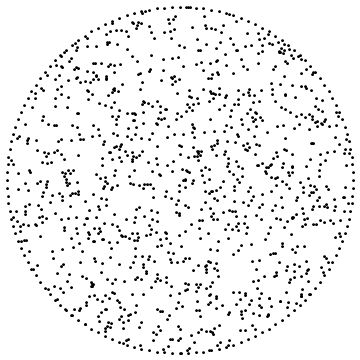
\includegraphics[scale=.38]{Graph1.png}}
\hfill
\subfloat[Using first algorithm]{\label{fig:Graph2}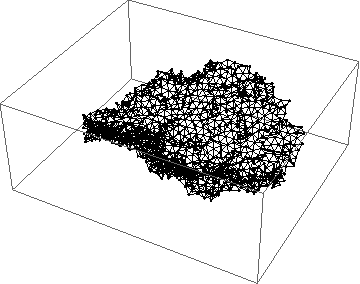
\includegraphics[scale=.40]{Graph2.png}}
\hfill
\subfloat[Using second algorithm]{\label{fig:Graph3}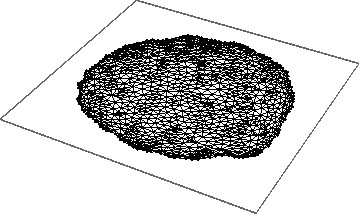
\includegraphics[scale=.40]{Graph3.png}}
\hspace{4mm}
\captionsetup{width=400pt}
\caption{Via a sprinkling into flat space, graphs can be obtained which are more or less flat.}
\label{fig:Graph1 and Graph2 and Graph3}
\end{center}
\end{figure}

The figure above shows a sprinkling into a flat space. The sprinkling is perfomed in a circular manner to reduce the peripheral effect, a known side-effect from spring embedders~\cite{Hu2005}. From this set of points, the relations are determined via Delaunay triangulation, which produces the dual graph of the Voronoi diagram. This procedure is very different from the way relations are established in the case of causal-sets. However, Delaunay triangulation is an easy way to produce partial orders which can be embedded into a Euclidean space. From the above sprinkling, graphs can be drawn using either of the two methods available in $Mathematica$. The result, in both cases, is a graph which look more or less flat, with some random fluctuations.

\begin{figure}[h]
\begin{center}
\subfloat[Curved space to sprinkle into]{\label{fig:Graph4}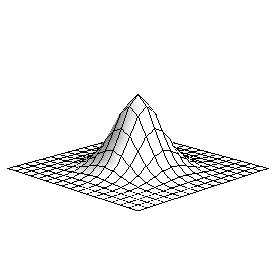
\includegraphics[scale=.7]{Graph4.png}}
\hspace{2cm}
\subfloat[The resulting sprinkling]{\label{fig:Graph5}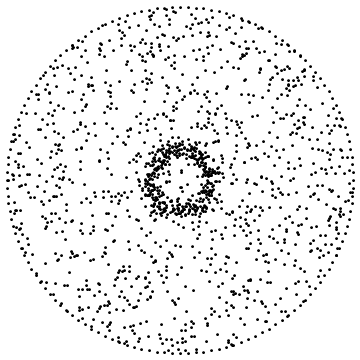
\includegraphics[scale=.45]{Graph5.png}}
\hspace{2mm}
\captionsetup{width=400pt}
\caption{By sprinkling into a curved space, there will be areas with a higher density of elements.}
\label{fig:Graph4 and Graph5}
\end{center}
\end{figure}

The sprinkling can also be performed in a curved space, such as the one depicted above. In this case, the density of elements is higher in the region where there is relatively more volume due to the curvature.

\begin{figure}[h]
\begin{center}
\subfloat[Using first algorithm]{\label{fig:Graph6}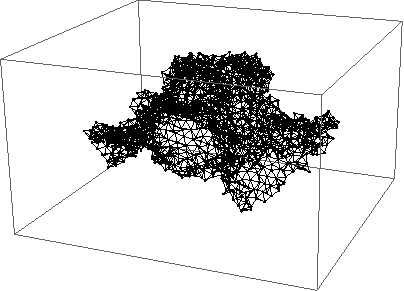
\includegraphics[scale=.51]{Graph6.png}}
\hfill
\subfloat[Using second algorithm]{\label{fig:Graph7}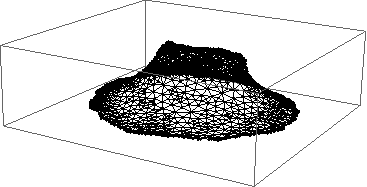
\includegraphics[scale=.6]{Graph7.png}}
\captionsetup{width=400pt}
\caption{The graphs from the curved space show the peculiar feature of the original space.}
\label{fig:Graph6 and Graph7}
\end{center}
\end{figure}

For such a sprinkling, the two algorithms produce graphs which clearly show a deviation away from flat space. In particular, we can identify the curvature-feature of the original space in both graphs.

\begin{figure}[h]
\begin{center}
\subfloat[Identified sprinkling]{\label{fig:Graph8}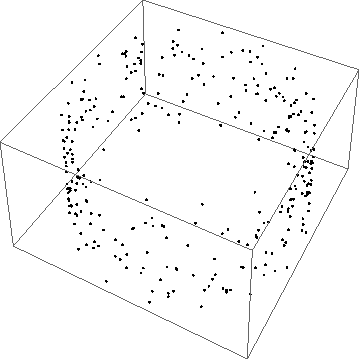
\includegraphics[scale=.4]{Graph8.png}}
\hfill
\subfloat[Using first algorithm]{\label{fig:Graph9}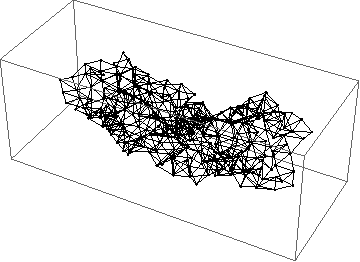
\includegraphics[scale=.4]{Graph9.png}}
\hfill
\subfloat[Using second algorithm]{\label{fig:Graph10}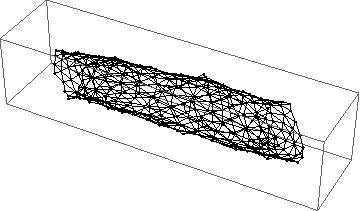
\includegraphics[scale=.4]{Graph10.png}}
\captionsetup{width=420pt}
\caption{By sprinkling into an identified space, the resulting graphs are cylindrical.}
\label{fig:Graph8 and Graph9 and Graph10}
\end{center}
\end{figure}

Finally, we can sprinkle into an identified space, a cylindrical space. The resulting graphs, obviously, show the compactification in the relations between elements. Each of the above cases show that a graph-drawing algorithm can deal with different types of sprinklings. For very large graphs, there is even a method which first coarse-grains the graph to produce a high-level structure, only to move on to lower-level structures in the second stage of the process~\cite{Hu2005}.

In the future, these algorithms may be extended to deal with Lorentzian distances. Then, they can serve as an easy way to retrieve coordinates for causal-set elements. There would even be a measure for the manifoldness of a causal-set. The total energy of the system is minimised during the process. Once in the steady-state, the remaining energy indicates how well the elements are capable of obtaining a volume of Planck size and a distance between linked neighbours of Planck size. As such, for a particular dimension, a low remaining energy means the causal-set is well embedded into the hyperspace.


\subsection{Interpolate a Function}
\label{sec:Interpolate a Function}

Once the coordinates within the hyperspace for every causal-set element are known, an interpolating function can be used to induce the metric. In particular, look at the graphs in figure~\ref{fig:Graph6 and Graph7}. The shape is very similar to figure~\ref{fig:Graph4}. If we interpolate a function $f$ through the points of the graph, this function will be very similar to the one originally used to perform the sprinkling. This interpolating function represents the embedding of the space into the hyperspace. Using this function, it is almost trivial to induce the metric.
\begin{equation}
\label{eq:Induced Metric}
g_{ab}=\left(\begin{array}{cc}
1+(\frac{\partial f}{\partial x})^2 & \frac{\partial f}{\partial x}\frac{\partial f}{\partial y}\\
\frac{\partial f}{\partial x}\frac{\partial f}{\partial y} & 1+(\frac{\partial f}{\partial y})^2
\end{array}\right)
\end{equation}
The procedure of inducing the metric can be extended to arbitrary dimensions, asuming the hypersurface is only one dimension higher than the space of interest.

%Dimension measure: The dimensions of an embedded causal-set is the dimension for which the spring-energy is low and adding 1 dimension does not significantly lower the energy. This is similar to SPSS lambda something. And the total energy is a measure of manifoldness. And Causal dynamical triangulations. 


%\section{More Causal-Set Technologies}
%\label{sec:More Causal-Set Technologies}
%\subsection{Classical Sequential Growth}
%\label{sec:Classical Sequential Growth}

%*This section might talk about the CSG model, just to fill up some more text in my dissertation.*
%\cite{Varadarajan2006} % Small update
%\cite{Rideout2002} % PhD version of original idea
%\cite{Rideout1999} % Original idea of CSG based on 3 contraints


%\subsection{Action}
%\label{sec:Action}

%*This section might talk about the action based on the d'Alembertian, just to fill up some more text in my dissertation.*
%\cite{Benincasa2010} % Introduces the 4D action
%\cite{Dowker2013} % nD action
%\cite{Benincasa2011} % action of different topologies, eg. cylinder


%\subsection{Swerves}
%\label{sec:Swerves}

%*This section might talk about the swerves model, just to fill up some more text in my dissertation.*
%\cite{Dowker2003} % Original swerves model with diffusion equation
%\cite{Philpott2009} % Update


%\subsection{Lambda Estimates}
%\label{sec:Lambda Estimates}

%*This section might talk about the prediction for lambda, just to fill up some more text in my dissertation.*
%\cite{Sorkin1997} % Original prediction for Lambda
\newpage
\section{Further Thoughts on Quantum Gravity}
\label{sec:Further Thoughts on Quantum Gravity}
\subsection{Deterministic Quantum Gravity}
\label{sec:Deterministic Quantum Gravity}

Most physicists would agree that quantum mechanics has proven the world is not deterministic. A model by 't Hooft, however, shows it may be possible that fundamentally deterministic laws of physics lie beneath the seemingly random quantum behaviour~\cite{Hooft1990}. In this case, the evolution operators are pure permutation matrices. 't Hooft claims that the quantum mechanical nature of the world can be attributed to an underlying law that is deterministic at the Planck scale but with chaotic effects at all larger scales. A model of a cellular automaton is constructed to demonstrate this new type of hidden variable theory. 't Hooft argues that hidden variable theories are generally not understood properly due to a misunderstanding of the notion of time in general relativity and should not immediately be discarded~\cite{Hooft1999}. One aspect which is needed for his model to work is that the world must be discrete. This is because a process of information loss is necessary and this is most easily attainable in a discrete theory. It would be interesting to see if causal-set theory, as one approach to a discrete theory of nature, can support a similar model to 't Hooft's.


\subsection{One Rule to Rule Them All}
\label{sec:One Rule to Rule Them All}

The idea that spacetime is a graph, or network, where links specify causal relations, is also a promiment feature of a theory by Wolfram. He proposes that these networks are grown via a simple set of rules based on the concept of a cellular automaton~\cite{Wolfram2002}. Particles are identified as specific sub-structures within the network. Like 't Hooft's idea, this model of spacetime is fully deterministic, and the randomness we currently observe is merely a build-up of chaotic behaviours since the early universe. A deterministic rule which dictates the growth of causal structures may also be applicable to causal-set theory~\cite{Bolognesi2010}. This fundamental rule, this one rule, would shape a faithfully embeddable causal-set where particles are particular instances of geometry. Curvature, then, results from the one rule reacting to such geometric sub-structures. One of the criticisms of Wolfram's idea is that it is not fully Lorentz invariant, nor does it respect Bell's causality~\cite{Aaronson2002}. As causal-set theory does not suffer from these theoretical issues, it may be interesting to see in what manner the two approaches can be combined.

\end{document}